%%%%%%%%%%%%%%%%%%%%%%%%%%%%%%%%%%%%%%%%%%%%%%%%%%%%%%%%%%%%%%%%%%%%%%%%%%%%%%%%%%%%%%%%%%%%%%%%%%%%%%%%%%%%%%%%%%%%%%%%%%%%%%%%%%%%%%%%%%%%%%%%%%%%%%%%%%%%%%%%%%%%%%%%%%%%%%%%%%%%
%%%%%%%%%%%%%%%%%%%%%%%%%%%%%%%%%%%%%%%%%%%%%%%%%%%%%%%%%%%%%%%%%%%%%%%%%%%%%%%%%%%%%%%%%%%%%%%%%%%%%%%%%%%%%%%%%%%%%%%%%%%%%%%%%%%%%%%%%%%%%%%%%%%%%%%%%%%%%%%%%%%%%%%%%%%%%%%%%%%%
%%%%%%%%%%%%%%%%%%%%%%%%%%%%%%%%%%%%%%%%%%%%%%%%%%%%%%%%%%%%%%%%%%%%%%%%%%%%%%%%%%%%%%%%%%%%%%%%%%%%%%%%%%%%%%%%%%%%%%%%%%%%%%%%%%%%%%%%%%%%%%%%%%%%%%%%%%%%%%%%%%%%%%%%%%%%%%%%%%%%
\FloatBarrier
\chapter{Improved dE/dx measurement for short tracks}
\label{sec:DeDxMeasurement}
As already pointed out in the previous chapter, the inclusion of the pixel energy measurements can increase the sensitivity when searching for short and highly ionising tracks.
While the energy measurements in the silicon strip detector have already been calibrated as part of the search for long-lived charged particles \cite{bib:CMS:HSCP_8TeV}, no complete calibration has been done for the pixel silicon tracker so far.
To increase the discrimination power of \dedx for short tracks, such a calibration procedure has therefore been performed within this PhD thesis.\\

The CMS tracker system provides a measurement of the particle's energy loss for each hit in the tracker.
This is done by the detection of the number of electrons produced by the ionisation of the silicon.
A detailed introduction to the CMS tracker system and the energy measurement can be found in Section~\ref{FIXME}.

How to combine the single energy measurements for each tracker hit into one track \dedx estimator that can be used for analysis purposes will be explained in the following Section~\ref{sec:sub:MeasuringDeDx}.
The pixel energy calibration is then described in Section~\ref{sec:EnergyCalibration}. 
How to discriminate SM particles and beyond SM particles with the help of a \dedx measurement is discussed in Section~\ref{sec:Ias}, followed by an exploration of how the inclusion of the pixel energy measurements in the \dedx estimates leads to a better discrimination between Standard Model particles and long-lived charginos (Section~\ref{sec:DiscriminationImprovements}).

%The CMS tracker system does not only allow for the precise measurement of particle tracks and primary and secondary vertices but also the measurement of a particle's mean energy loss per path length.
%This is done by the detection of the number of electrons produced by the ionisation of the particle during its passage through the silicon tracker.
%A detailed introduction to the CMS tracker system and the energy measurement can be found in Section~\ref{}.

%It was already pointed out that the inclusion of the pixel energy measurements can increase the sensitivity when searching for short and highly ionising tracks.
%While the silicon strip detector has already been calibrated as part of the search for long-lived charged particles \cite{bib:CMS:HSCP_8TeV}, no complete calibration has been done for the pixel silicon tracker so far.
%To increase the discrimination power of \dedx for short tracks, such a calibration procedure is therefore conducted within this PHD thesis.


\section{Estimation of the ionisation loss of charged particles}
\label{sec:sub:MeasuringDeDx}
Energy losses for moderately relativistic charged particles travelling through matter are mostly caused by ionisation effects.
The mean energy loss per path length can be described with the Bethe formula \cite{bib:Bethe_1930}:
\begin{equation}
\langle \frac{dE}{dx} \rangle = Kz^2\frac{Z}{A}\frac{1}{\beta^2} [ \frac{1}{2} \ln{\frac{2m_e c^2 \beta^2 \gamma^2 T_{\text{max}}}{I^2}} - \beta^2 - \frac{\delta( \beta \gamma )}{2} ].
\end{equation}
It is a function of the atomic number ($Z$), the atomic mass ($A$) of the absorber, and the mean excitation energy ($I$) which is 173\,eV for silicon~\cite{bib:NIST}.  
$T_{\text{max}}$ represents the maximum energy transfer in a single collision.
The relevant particle's properties are the velocity ($\beta$), the Lorentz factor ($\gamma$) and the charge (z) of the incident particle.
The density correction $\delta( \beta \gamma )$ reduces the mean energy loss at high energies because of polarisation effects of the material. 
%The constant factor K is $4\pi N_A r_e^2 m_e^2 c^2$ with $N_A$ being the Avogadro constant, $m_e$ the electron mass and $r_e$ the classical electron radius of 2.8\,fm.
The factor K is constant and is 0.307 in units of $\mev\,$mol$^{-1}$cm$^2$.
The Bethe formula is valid if the main energy loss originates from ionisation effects, \ie in a region between $0.1\lesssim\beta\gamma\lesssim 1000$.


Even if widely used, the mean energy loss is a quantity which is ``ill-defined experimentally and is not useful for describing energy loss by single particles'' \cite{bib:PDG_2014}.
The problem is caused by the underlying probability distribution of one single \dedx measurement (this will be named $\Delta E/ \Delta x $ throughout the following sections), which can be parametrised by a Landau distribution \cite{bib:Landau_1944}
\begin{equation}
p(x) = \frac{1}{\pi} \int_0^\infty\! e^{-t \log t - x t} \sin(\pi t)\, dt.
\end{equation}
The Landau distribution has no free parameters. Its most probable value is around 0.222.
However, it is possible to introduce artificially a different most probable value and a width (at half maximum) with $x \rightarrow \frac{x-\text{MPV}}{\sigma}-0.222$.
The Landau distribution is a highly asymmetric distribution with a long tail towards large $x$ values (see Fig.~\ref{fig:landau}).
\begin{figure}[!t]
  \centering 
  \begin{tabular}{c}
  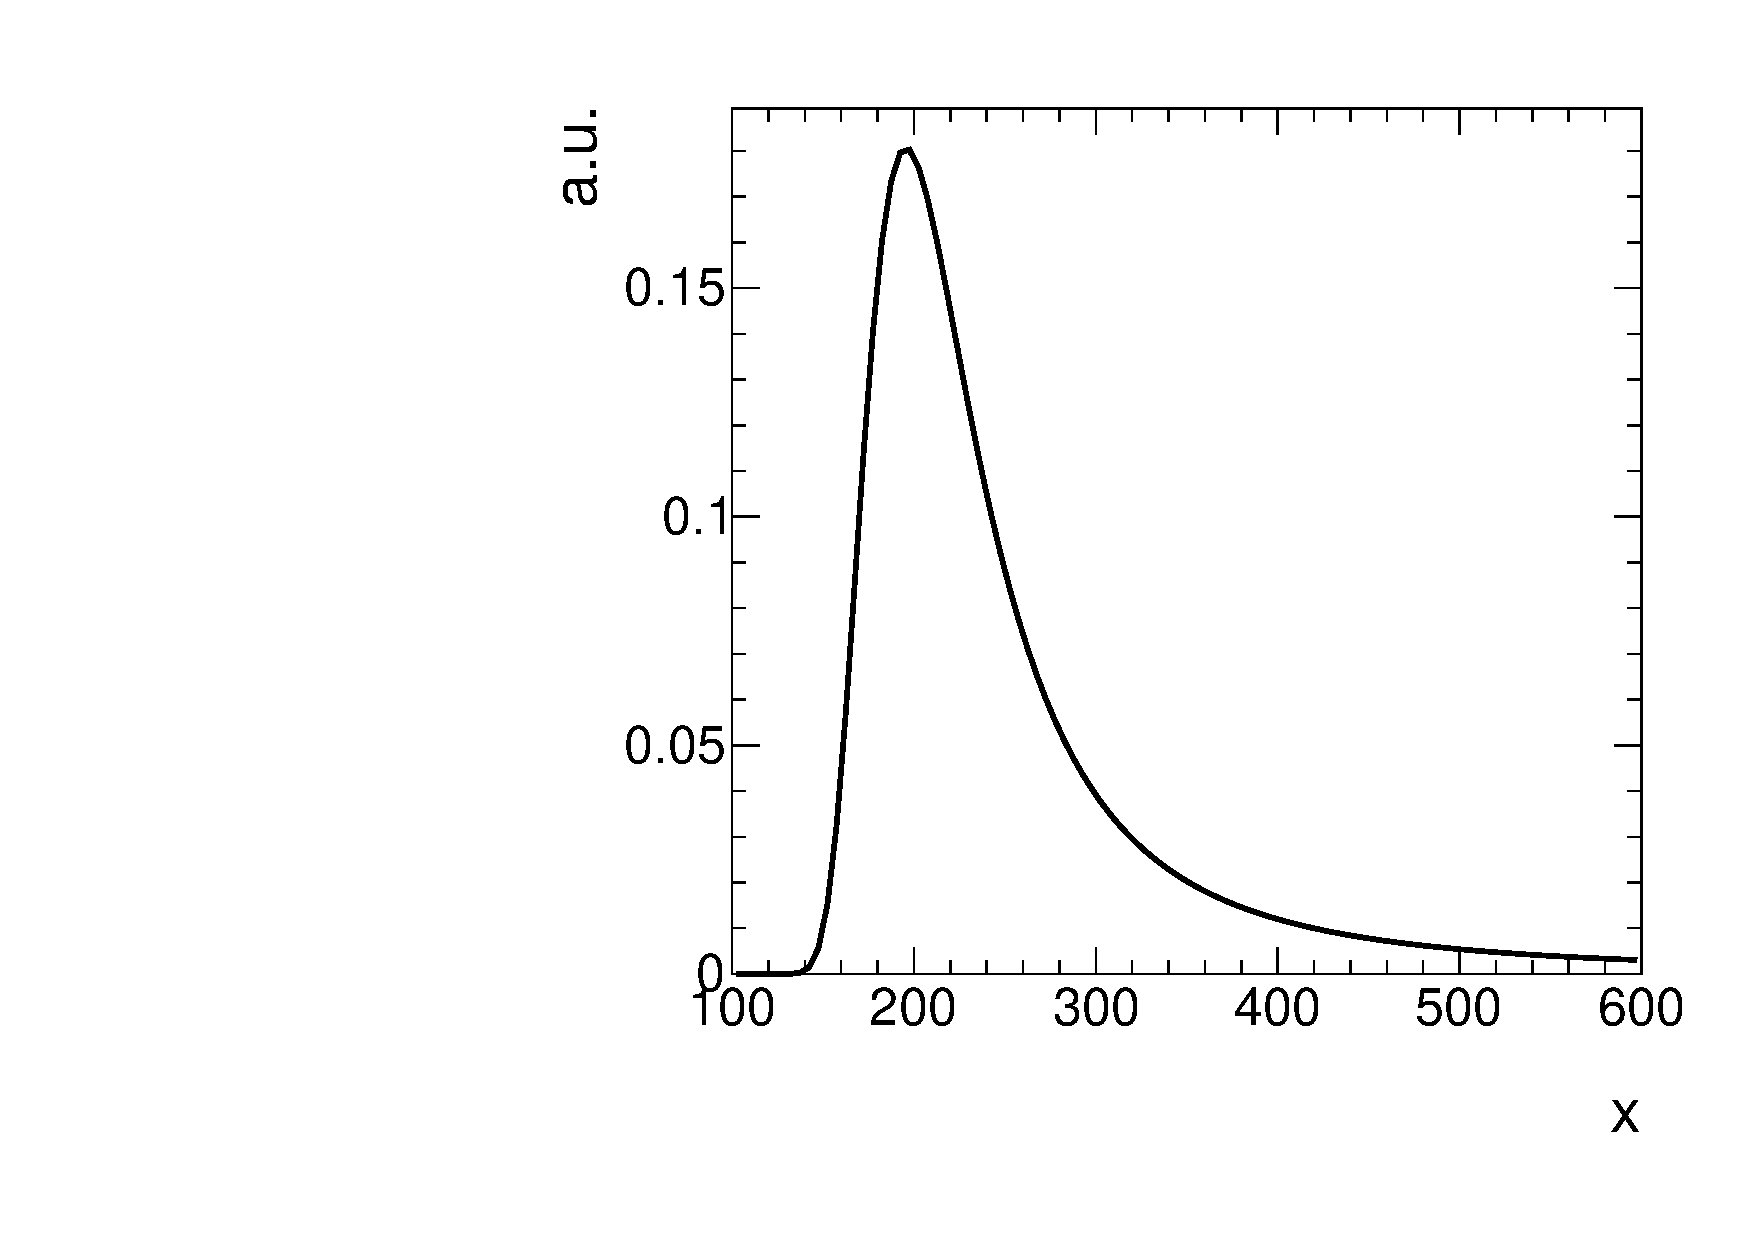
\includegraphics[width=0.49\textwidth]{figures/analysis/PixelCalibration/Landau.pdf}
  \end{tabular}
  \caption{Illustration of the shape of a Landau distribution. Parameters were chosen as $\mu=200$ and $\sigma=20$.} 
  \label{fig:landau}
\end{figure}
Theoretically it extends to infinite energies, however in nature the maximal deposited energy is of course limited by the particle's full energy.
%The mean and the variance of a landau distribution are not defined.

Because of its strong asymmetry, measurements of the mean energy loss per path length $\langle \dedx \rangle$ with only a few single measurements are easily fluctuating towards high values.
This makes the use of the mean energy loss described by the Bethe formula for the discrimination of new heavy particles problematic, because fluctuations to high values reduce the discrimination power against massive particles which release in general higher amounts of energy in matter.
%This is again different for a (limited) measurment, as there it is always possible to calucalute a mean.
%Still, this leads to the fact that the definition of the mean energy loss per path length is a problematic and unstable concept.


A much better observable is the most probable value (MPV) of the Landau distribution.
The MPV is much more stable compared to the mean and is not subject to high \dedx fluctuations. 
The most probable energy loss of a charged particle, $\Delta_p$, can be described by the Landau-Vavilov-Bichsel equation \cite{bib:Bichsel:MPV_1988}:
\begin{equation}
\Delta_p = \xi \left[ \ln \frac{2m_e c^2\beta^2\gamma^2}{I}  + \ln\frac{\xi}{I} + j - \beta^2 - \delta(\beta\gamma)  \right],
\label{eq:Landau_Vavilov_Bichsel}
\end{equation}
with $\xi=(K/Z)\langle Z/A \rangle (x/\beta^2)$. 
The thickness of the absorber $x$ appears explicitly in the Landau-Vavilov-Bichsel equation making the most probable energy loss per path \mbox{length $\Delta_p/dx$} logarithmically dependent on $x$.
A comparison between the Bethe mean energy loss $\langle \dedx \rangle$ and the most probable energy loss $\Delta_p/dx$ for muons is shown in Fig.~\ref{fig:dEdx_Bethe_Landau}.

%However, it is difficult to determine the most probable value for tracks with only a few energy measurements available.
%Large fluctuations can still lead to a bias towards higher value of the most probable \dedx.

Particles such as  muons are minimally ionising in silicon for $\beta\gamma \sim 3-4$. 
For higher momenta the deposited energies increase again reaching a plateau at around $\beta\gamma\sim100$. 
However, new heavy charged particles would mainly be unrelativistic because of their high mass and would therefore deposit much higher energies in the detector.
This makes \dedx  a very well discriminating variable.
%\begin{figure}[!bt]
%  \centering 
%  \begin{tabular}{c}
%  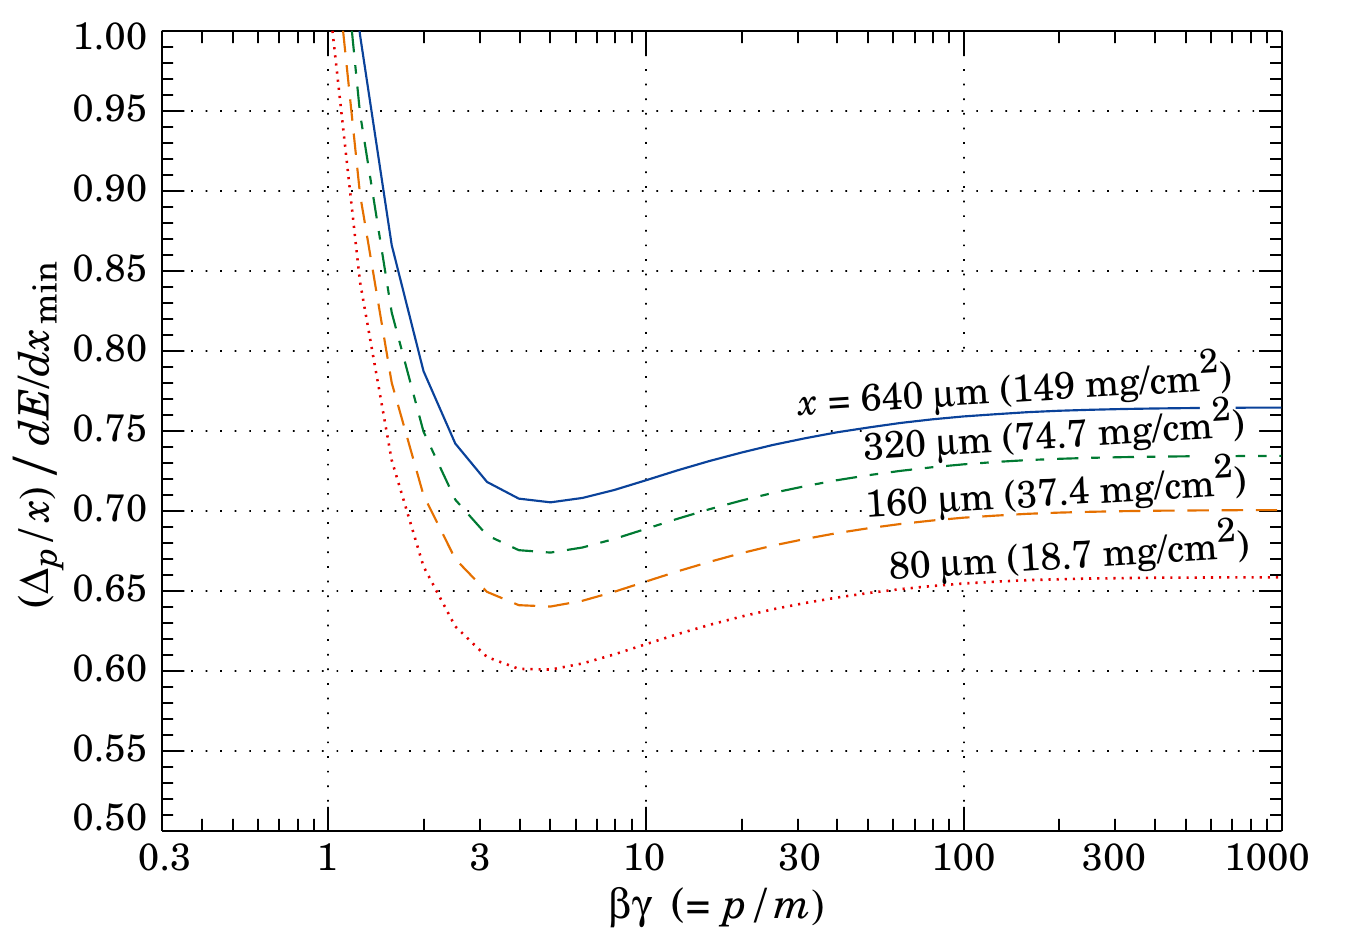
\includegraphics[width=0.6\textwidth]{figures/analysis/dEdx_Landau_Silicon.png}
%  \end{tabular}
%  \caption{Most probable energy loss in silicon, scaled to the mean loss of a minimally ionising particle (388 eV/$\mu$m) for different absorber thicknesses. Taken from \cite{bib:PDG_2014}.} 
%  \label{fig:dEdx_Landau_Silicon}
%\end{figure}
\begin{figure}[!t]
  \centering 
  \begin{tabular}{c}
  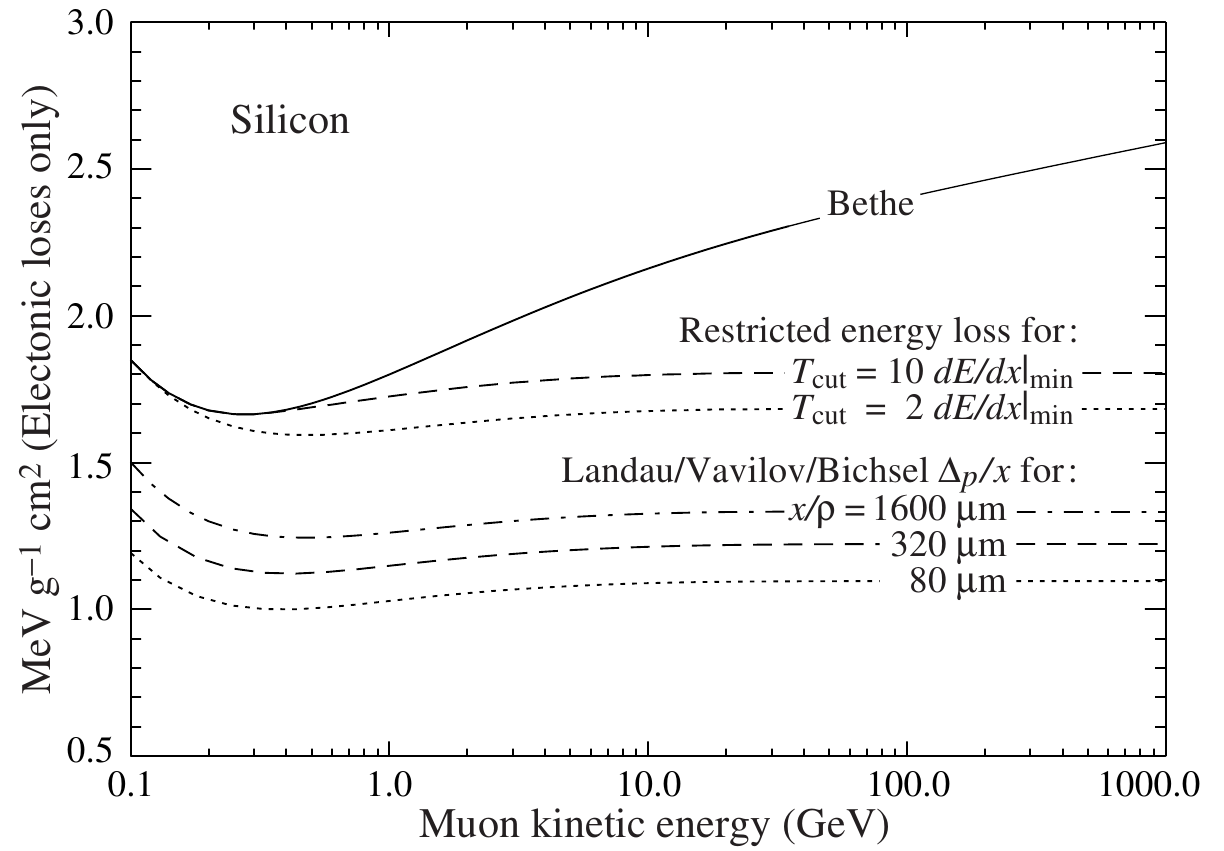
\includegraphics[width=0.6\textwidth]{figures/analysis/dEdx_Bethe_Landau.png}
  \end{tabular}
  \caption{Comparison between the Bethe mean energy loss, restricted energy loss and the most probable energy loss described by the Landau-Vavilov-Bichsel function for muons for different values of absorber thickness of silicon. Taken from \cite{bib:PDG_2014}.} 
  \label{fig:dEdx_Bethe_Landau}
\end{figure}
Thus, the energy loss per path length can be used to discriminate between SM particles and new heavy charged particles due to the different velocity distributions.\\



As said before, the most probable energy loss is much more stable compared to the Bethe mean energy loss.
Still, combining only a few measurements of $\Delta E/\Delta x$ can also lead for $\Delta_p/dx$ to large fluctuations towards high \dedx values.
In order to estimate experimentally the most probable \dedx value from only a few energy measurements, several ``estimators'' can be used that suppress a potential bias towards the high end without introducing a bias towards lower values~\cite{bib:Quertenmont_2010}.
One of the estimators for determining a track's \dedx is the harmonic-2 estimator
\begin{equation}
\ihtwo=\left( \frac{1}{N}\sum_{i=1}^{N}(\Delta E_i/\Delta x_i)^{-2} \right)^{-1/2},
\label{eq:Harmonic2Estimator}
\end{equation}
where $\Delta E_i /\Delta x_i$ corresponds to the $\Delta E$ and $\Delta x$ measurement in the $i$th hit of the track. 
This estimator is known to be robust and is not easily biased by large fluctuations in  $\Delta E/\Delta x$ because of the suppression by the power of minus two~\cite{bib:Quertenmont_2010}.
%The harmonic mean of all $N$ measurements to the power of two is used as estimator for the MPV of the \dedx distribution of a particle.

A further estimator of \dedx used for the discrimination of highly ionising particles will be introduced in Section~\ref{sec:Ias}.


\FloatBarrier
\section{Energy calibration of the silicon pixel tracker}
\label{sec:EnergyCalibration}
During Run I in 2012, the pixel silicon detector was continuously subjected to an energy calibration, a so-called gain calibration.
Every pixel was calibrated to the same response, so that the whole pixel tracker should have been well inter-calibrated~\cite{bib:Danek}.
Unfortunately, due to various reasons, such as the imperfect constancy of the reference signal, or radiation and temperature induced changes, the energy calibration could not ensure a fully calibrated pixel tracker.
%was not adequate enough to use the measured energy deposition without a further offline calibration procedure.

This imperfection of the gain calibration can be seen in Fig.~\ref{fig:StabilityPlot_beforeCalibration}, where the mean of the harmonic-2 estimator for all tracks $\langle\ihtwo \rangle$ over the full data-taking period in 2012 is shown.
Four different steps can be spotted.
\begin{figure}[!b]
  \centering 
  \begin{tabular}{c}
  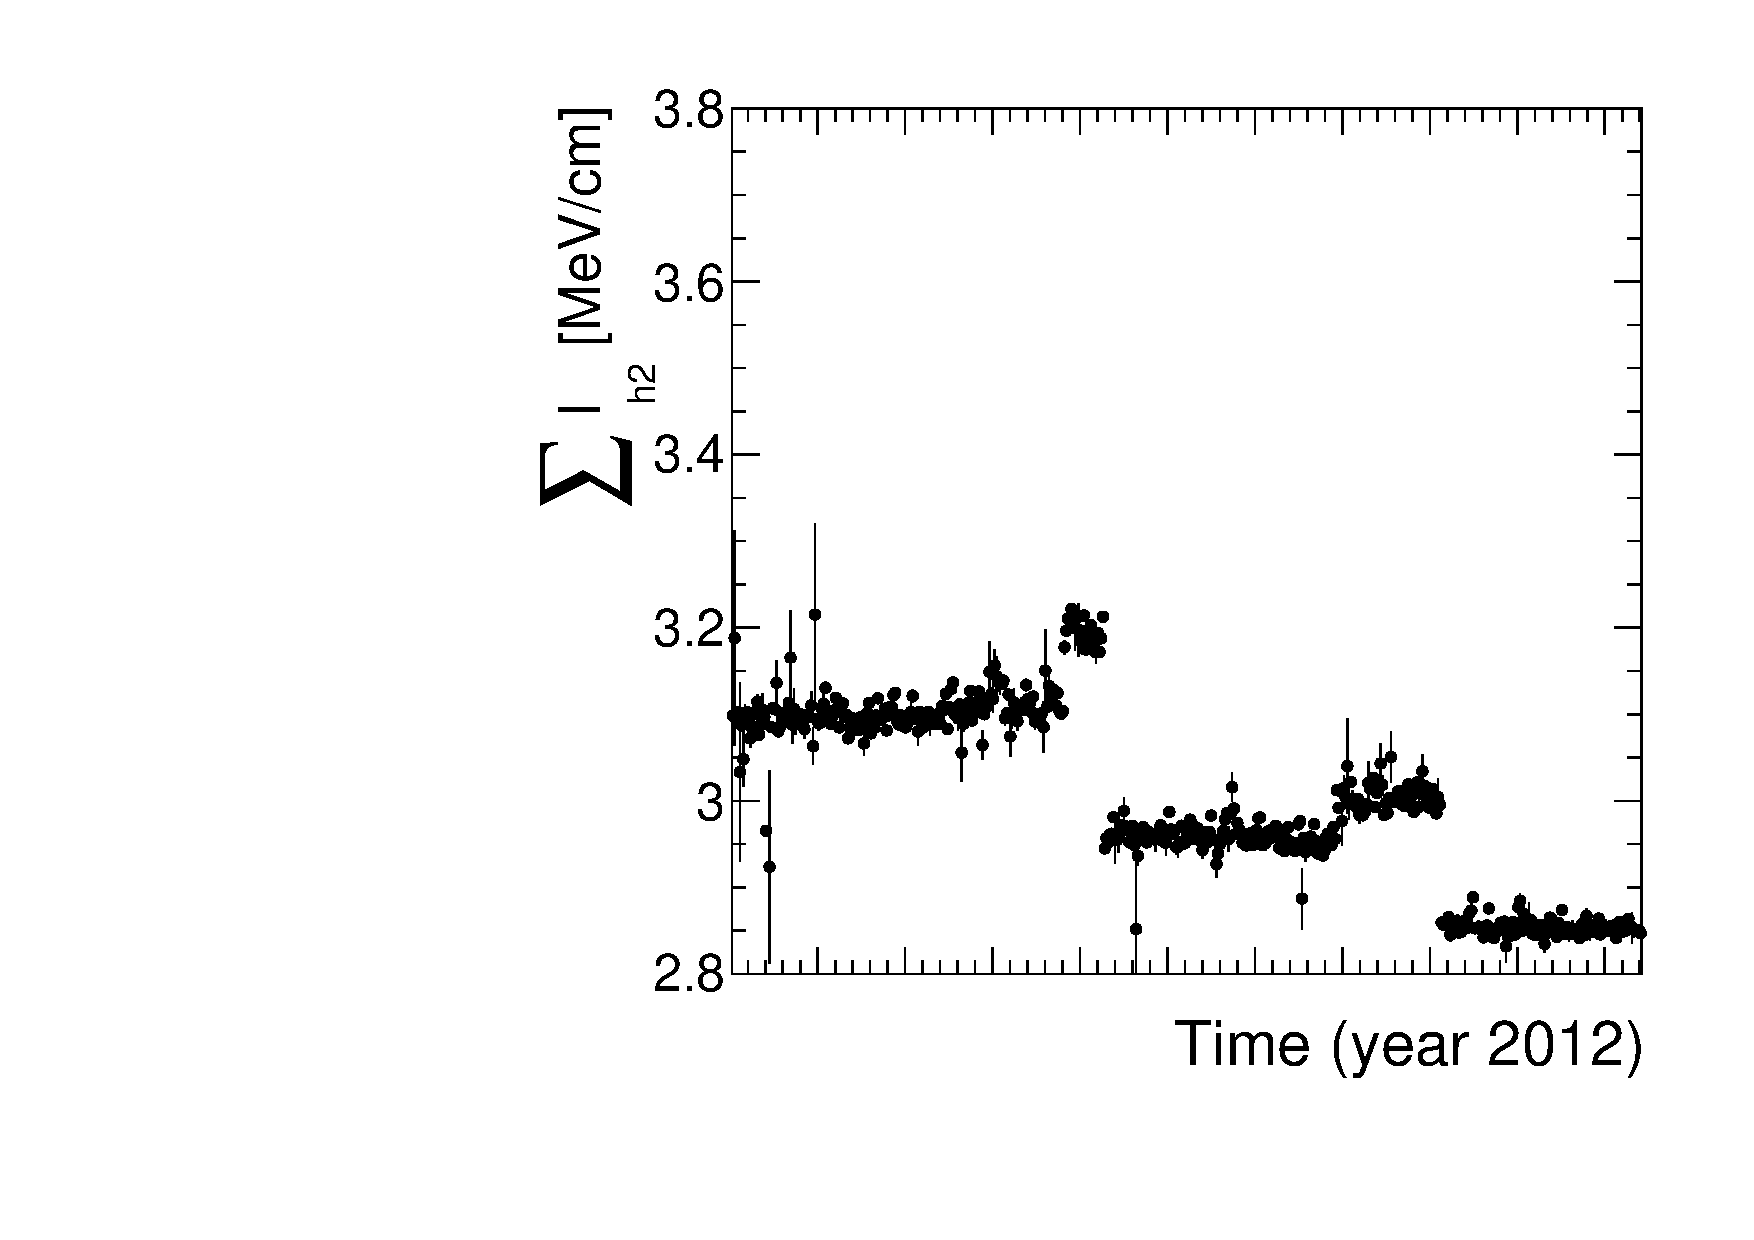
\includegraphics[width=0.49\textwidth]{figures/analysis/PixelCalibration/StabilityPlot_Pixel_beforeCalibration_withoutStepFits_NEW.pdf}
  \end{tabular}
  \caption{Mean of all track's \dedx (harmonic-2 estimator) over the full year 2012. Only pixel hits are taken into account. Every data point corresponds to one run.} 
  \label{fig:StabilityPlot_beforeCalibration}
\end{figure}
The first and the third steps correspond to changes in the settings of the tracker due to irradiation.
The second and fourth step are induced by associated adjustments in the online gain calibration.
Unfortunately, although the gain calibration was adjusted (even with some delay), it was not able to ensure a constant energy response of the pixel tracker over time. 
The variations of the \dedx measurement over time of around 15\% are too large to use \dedx without a further calibration. 

The following sections explain the method of the gain calibration of the pixel silicon tracker which is performed for this analysis. 
It is splitted into two sections. 
The first section is dedicated to the gain inter-calibration of the pixel tracker which ensures a homogeneous energy response of all tracker modules.
In the second section, the absolute gain calibration is discussed. 
This calibration step is needed to ensure that the measurement of the energy release of a particle is actually translated to the correct physical value.

%Detailed technical information about the pixel tracker can be found in Section~\ref{sec:Detector:Pixel}.


\subsection*{Inter-calibration of gain}
The main goal of the gain calibration is to get a uniform response in the ionisation energy loss \dedx over the full data taking period in 2012.
To also ensure a uniform response over all modules within one time step, an additional inter-calibration on module level is carried out.
The inter-calibration can in principle be done on various levels: the highest granularity would be a calibration on pixel level, followed by a calibration on read-out-chip (ROC) level and then on module-level.
Lower granularities in descending order are rings (modules with same z-position) and finally layers (3 layers in the barrel and 4 disks in the endcap). 
Within this anlysis the calibration is performed on module level because ROCs within one module are acceptably calibrated within 10\% (Fig.~\ref{fig:SigmaPixelCalibrationROCs} in Appendix~\ref{app:PixelCalibration}) while discrepancies larger than 20\% frequently and up to 100\% occur on module level (Fig.~\ref{fig:PixelCalibrationFactors} in Appendix~\ref{app:PixelCalibration}).

%The applied method for the gain calibration of the pixel tracker closely follows the method in \cite{bib:Quertenmont_2010}.

The gain calibration of the pixel silicon tracker is carried out with the help of minimally ionising particles (MIPs).
MIPs in this context are not defined as particles at the minimum of the Bethe formula, but more generally as particles located at or near the plateau of the \dedx distribution vs. momentum (see Fig.~\ref{fig:dEdx_Bethe_Landau}).
This approach ensures that all particles deposit similar amounts of energy so that the variation due to different momenta is minimised.

MIPs are selected by a momentum selection of $\text{p}>2\,$\gev.
Additionally, only tracks with at least eight hits and a $\chi^2/\text{n.d.o.f.}<3$ are used to ensure a high-quality track reconstruction.
A sample containing around $~$50 million ``minimum bias'' events is used for calibration.
The ``minimum bias'' sample was specifically recorded for tracker calibration purposes.
%Its distinctive property is that neither an online nor offline selection was applied.

For every module in the pixel tracker (there are 1440 modules in total), a distribution of the energy loss per path length $\Delta E/\Delta x$ is built.
The measurement of $\Delta E/\Delta x$ is done in ADC counts per mm.
ADC counts are a measure for the deposited charge after digitisation.
%each $\Delta E/\Delta x$  measurement of all particles crossing the module is filled into a histogram. 
Figure~\ref{fig:dEdx_Module} shows an example distribution for one module. 
\begin{figure}[!t]
  \centering 
  \begin{tabular}{c}
  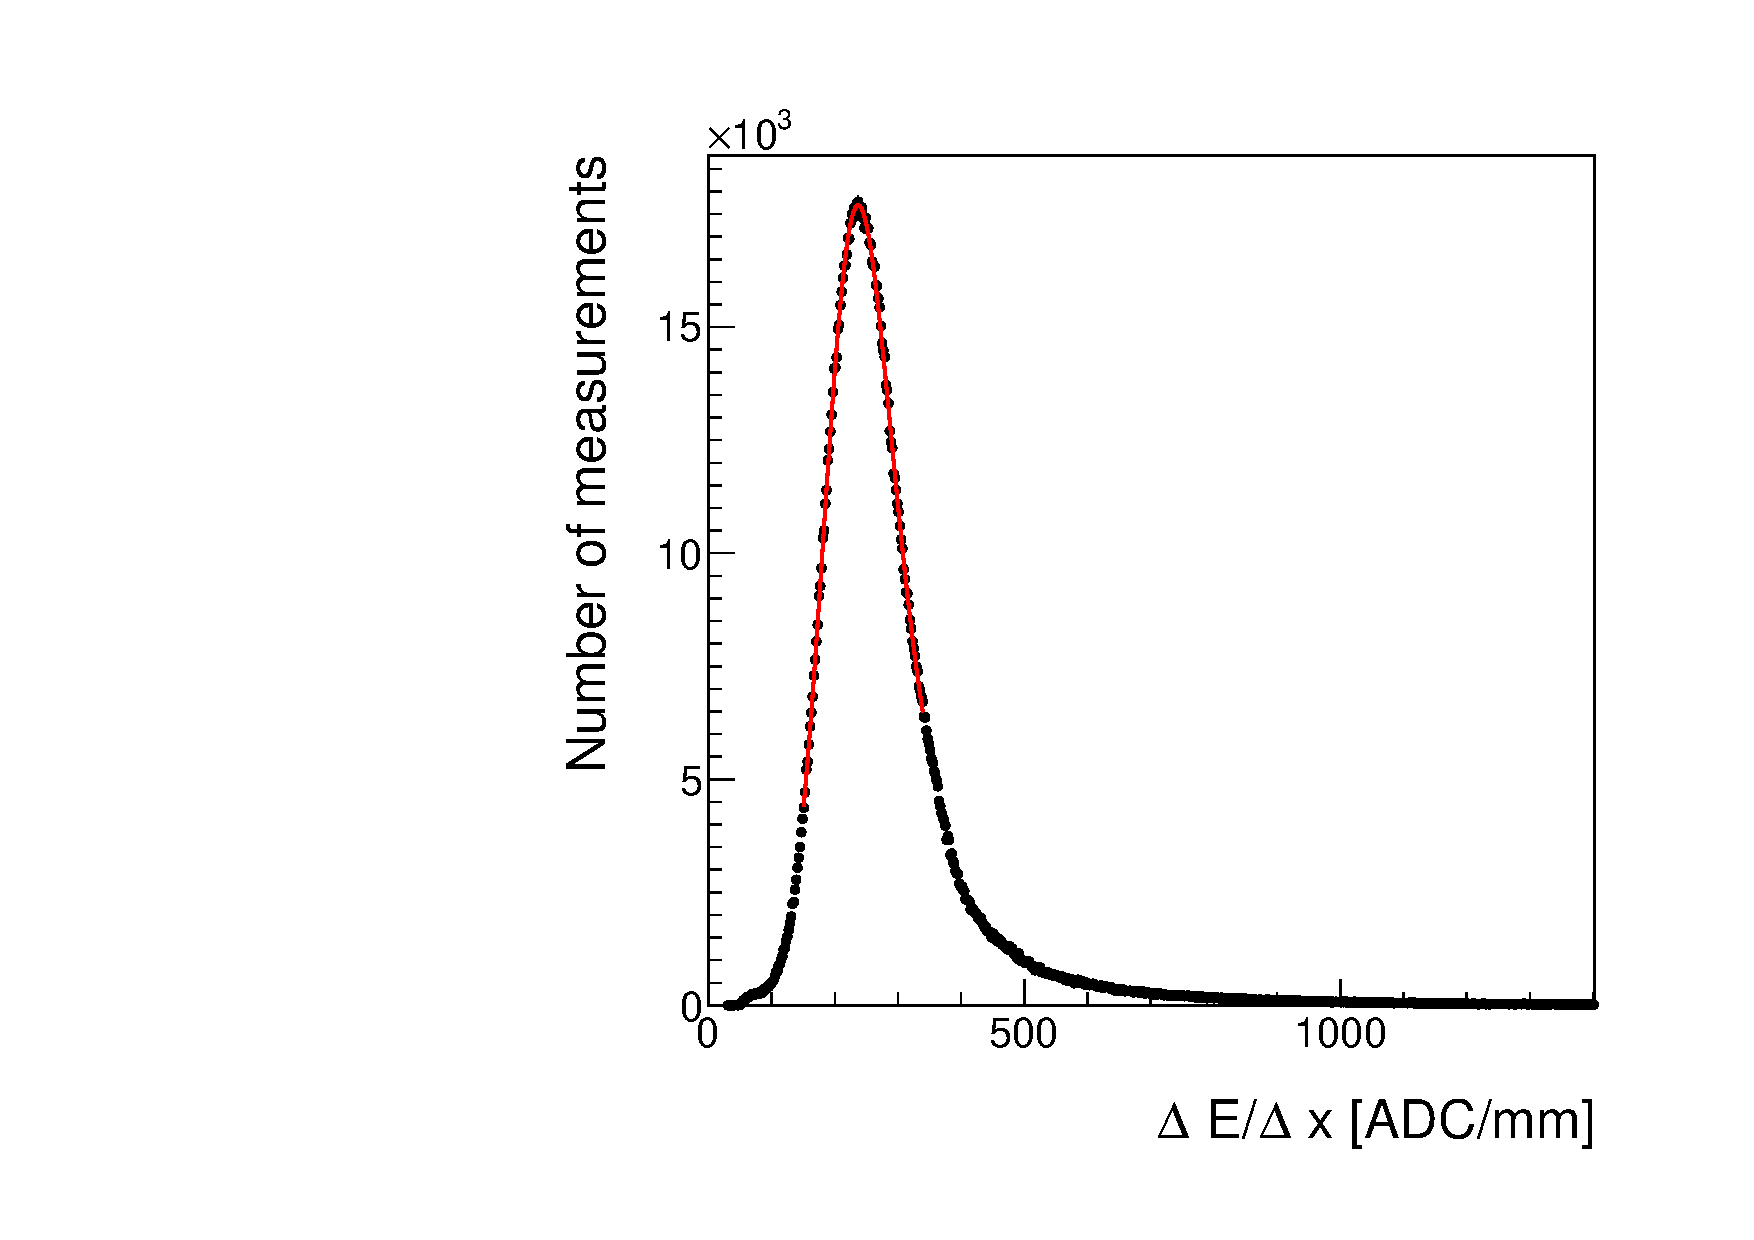
\includegraphics[width=0.49\textwidth]{figures/analysis/Landau_Module_352476680.pdf}
  \end{tabular}
  \caption{An example of the $\Delta E/\Delta x$ distribution measured in ADC count per mm for one module of the CMS pixel tracker. 
           A Landau convoluted with a Gaussian is fitted to the core of the distribution in an iterative procedure.} 
  \label{fig:dEdx_Module}
\end{figure}
To extract the MPV for every module a fit to the core distribution is performed.
The fit is not only done with a Landau but a Landau convoluted with a Gaussian function to be closer to the experimentally observed energy spectrum.
This also increases the fit performance and the stability of the fit.
The path length $\Delta x$ is calculated with
\begin{equation}
\Delta x = d_{\text{module}_i} \cdot \cos(\phi_{\text{track}}),
\end{equation}
where $d_{\text{module}_i}$ is the thickness of module i and $\phi_{\text{track}}$ is the relative angle of the particle's trajectory to the normal axis of the module.
With the measured MPV extracted from the fit, an inter-calibration factor is calculated for every module
\begin{equation}
c_{\text{inter}}=\frac{\mpv_{\text{target}}\, [\text{ADC/mm}]}{\mpv\, [\text{ADC/mm}]} = \frac{300 \cdot 265 \, \text{ADC/mm}}{\mpv\, [\text{ADC/mm}]}.
\end{equation}
The factor 300 $\cdot$ 265 ADC/mm is in principal an arbitrary number since the final response is adjusted by the absolute gain calibration described in the next section.
However, it is chosen such that the measured calibration factors are close to one.
The calibration factor can then be used to scale every single measurement in a module to a calibrated $\Delta E/\Delta x$ measurement
\begin{equation}
\left( \frac{\Delta E}{\Delta x}\right)_{\text{calibrated}}=c_{\text{inter}} \cdot \left(\frac{\Delta E}{\Delta x}\right)_{\text{uncalibrated}}
\end{equation}
The determination of the calibration factor is done for every of the five time steps, shown in Fig.~\ref{fig:StabilityPlot_beforeCalibration} independently, in order to get rid of the time dependency. 
The outcome of the application of the calibration factors to the single energy measurements in the pixel tracker can be seen in Fig.~\ref{fig:StabilityPlot_afterCalibration}.
The variation over time is indeed eliminated, resulting in a maximal time variation of less than $\sim1$\%.

\begin{figure}[!t]
  \centering 
  \begin{tabular}{c}
  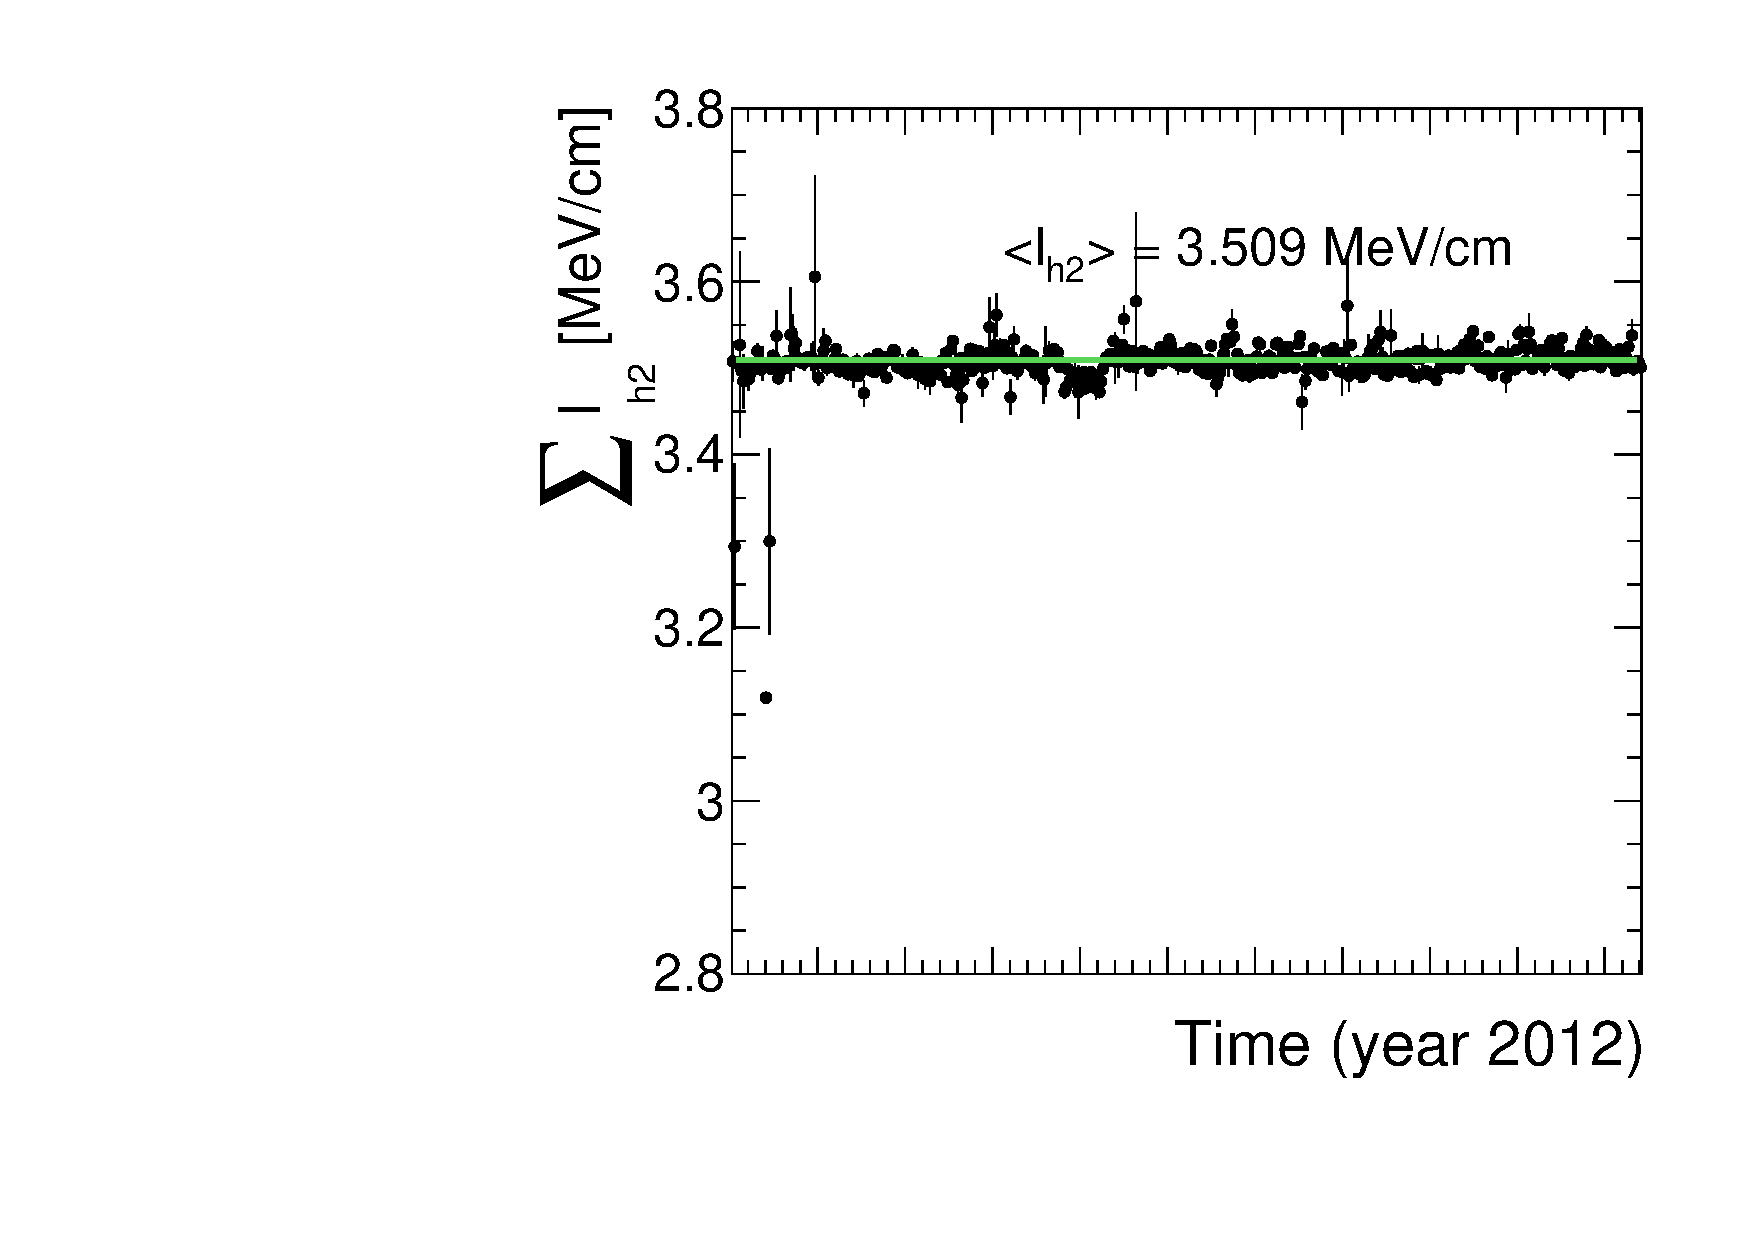
\includegraphics[width=0.49\textwidth]{figures/analysis/PixelCalibration/StabilityPlot_Pixel_afterCalibration_withoutStepFits_NEW.pdf}
  \end{tabular}
  \caption{Mean of all track's \dedx (harmonic-2 estimator) over the full year 2012 after applying the calibration factors, resulting in an average \dedx of 3.51 MeV/cm. Only pixel hits are taken into account. Every data point corresponds to one run.} 
  \label{fig:StabilityPlot_afterCalibration}
\end{figure}

Additionally, the same procedure is carried out for a corresponding simulated data sample to ensure the inter-calibration of the pixel modules on all simulated samples.



\subsection*{Absolute calibration of gain}
As a final step, the targeted \mpv being $\mpv_{\text{target}}=300 \cdot 265 \,  \text{ADC/mm}$ needs to be translated to a meaningful physical quantity given in physical units (\eg MeV/cm).
That means, that the charge measurement in ADC counts needs to be converted to the real energy release from a particle.
The relation between $\Delta E$ in ADC counts and the energy loss in eV is given by
\begin{equation}
\Delta E\,[\ev] = c_{\text{inter}} \cdot \Delta E\,[\text{ADC}] \cdot \frac{N_e}{\text{ADC}} \cdot 3.61 \, \ev,
\end{equation}
where $N_e$/ADC is the number of electrons which correspond to one calibrated ADC count and 3.61\,\ev is the  mean energy needed to create one electron-hole pair in silicon at $-10\degree$C.
Such an absolute gain calibration can be done with the help of several methods (all explained in \cite{bib:Quertenmont_2010}).
The absolute calibration of the silicon pixel tracker can rely on the existing absolute calibration of the silicon strip detector.
In \cite{bib:Quertenmont_2010}, the absolute gain calibration was done with the help of the most probable energy release per path length of muons, 
theoretically described by the Landau-Vavilov-Bichsel formula in Eq.~\eqref{eq:Landau_Vavilov_Bichsel}.  
To calibrate the pixel tracker to the correct energy loss per path length it is therefore sufficient to determine one calibration factor to relate the average \dedx of all tracks in the pixel tracker as shown in 
Fig.~\ref{fig:StabilityPlot_afterCalibration} to the average measured \dedx in the strip tracker, shown in Fig.~\ref{fig:StabilityPlot_Strip} by
\begin{equation}
c_{\text{absolute}} = \frac{\langle dE/dx_{\text{strip}} \rangle}{\langle dE/dx_{\text{pixel}} \rangle} = \frac{3.303}{3.509} = 0.941.
\end{equation}
\begin{figure}[!t]
  \centering 
  \begin{tabular}{c}
  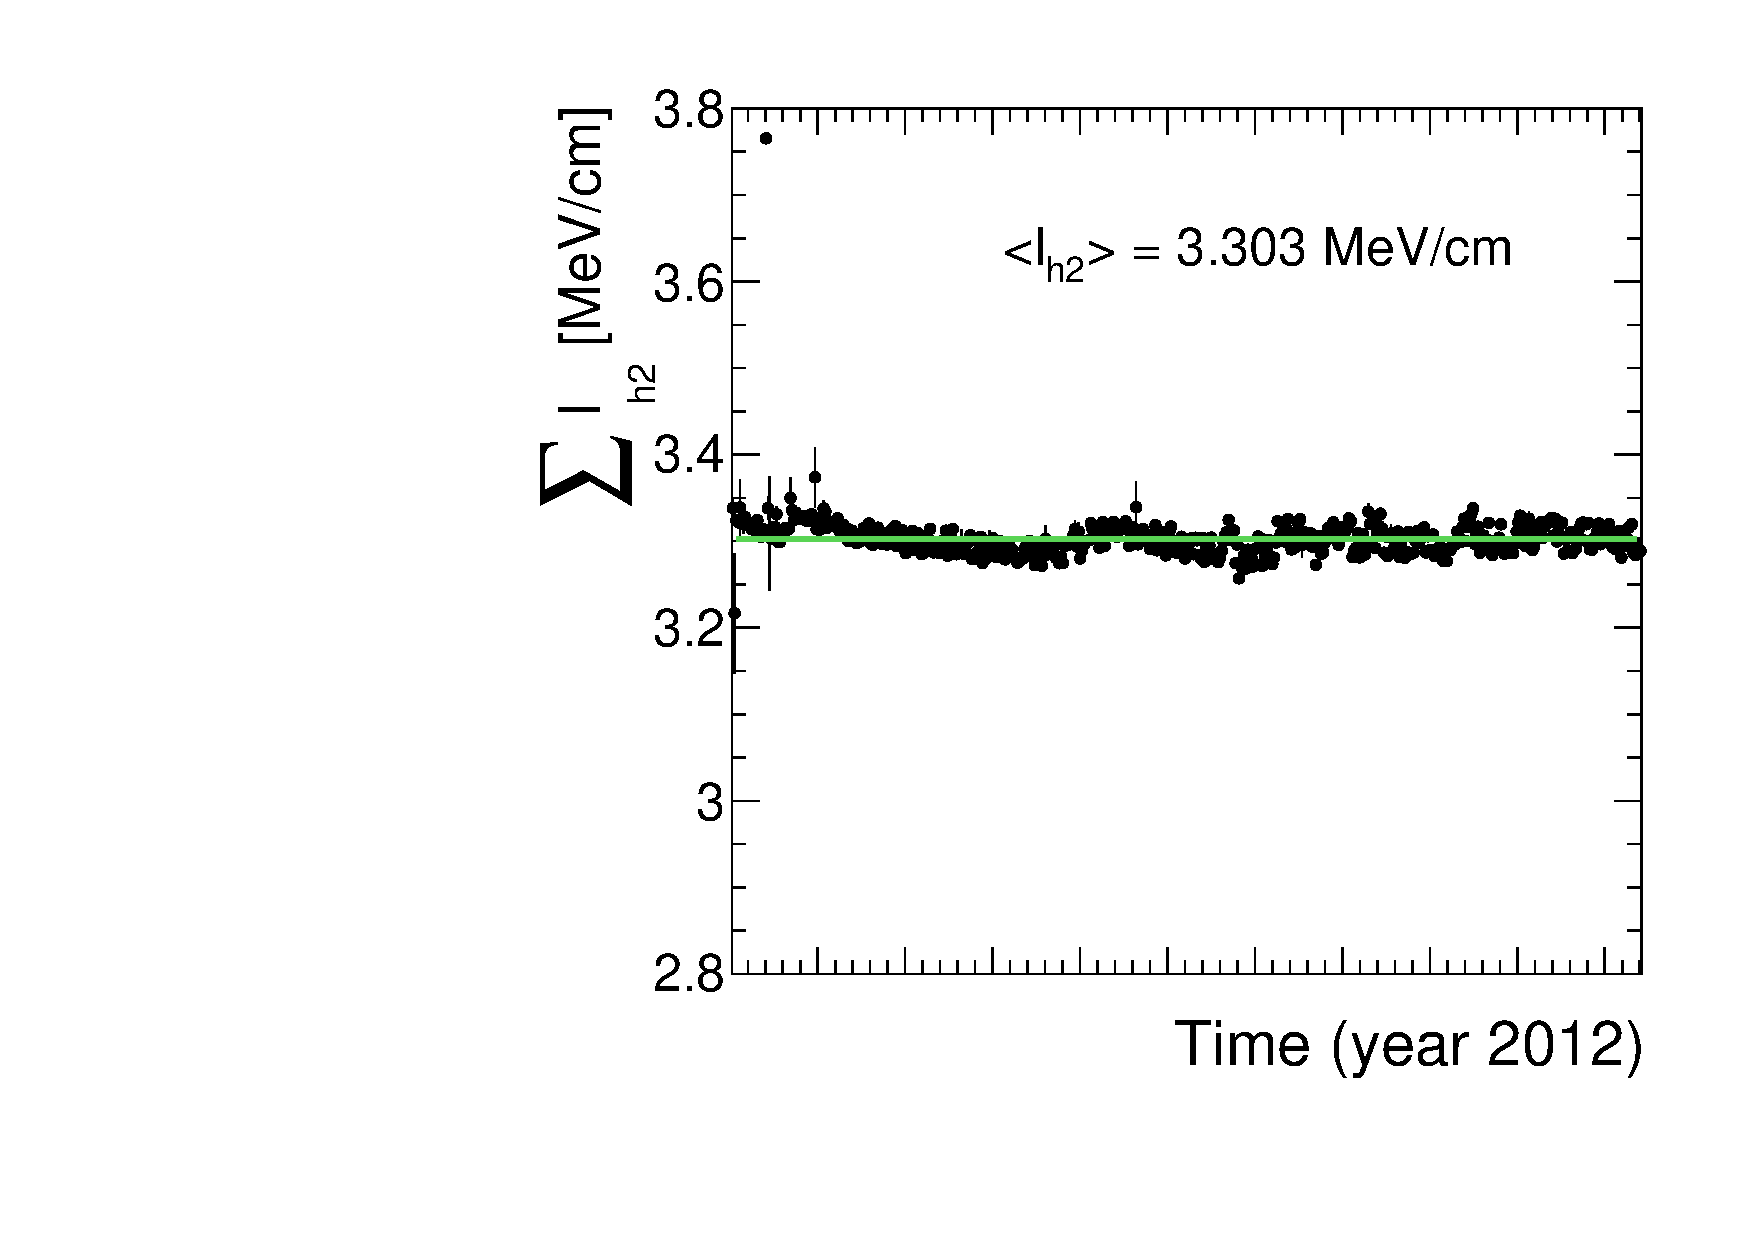
\includegraphics[width=0.49\textwidth]{figures/analysis/PixelCalibration/StabilityPlot_Strip_afterCalibration_withoutStepFits_NEW.pdf}
  \end{tabular}
  \caption{Mean of all track's \dedx (harmonic-2 estimator) measured in the silicon strip detector over the full year 2012. The average most probable \dedx is $\ihtwo=3.303\,\mev/\cm$. Every data point corresponds to one run.} 
  \label{fig:StabilityPlot_Strip}
\end{figure}
This factor is then applied on top of $c_{\text{inter}}$ for all pixel modules.

Finally, an absolute calibration factor needs to be determined for the simulated samples, where the simulated pixel tracker is calibrated to the average \dedx of the silicon strip measured in data.


\section{Discrimination of highly-ionising particles}
\label{sec:Ias}

As mentioned before, it is difficult to find a robust estimator for the most probable energy loss of a particle, if only a few measurements of $\Delta E/ \Delta x$  along the particle's trajectory are available.
The harmonic-2 estimator \ihtwo was already introduced in Section~\ref{sec:sub:MeasuringDeDx} in Eq.~\eqref{eq:Harmonic2Estimator}.
It is known to be a robust estimator not easily affected by large fluctuations in $\Delta E/ \Delta x$.
However, it was shown in \cite{bib:Quertenmont_2010} that a better discrimination between SM particles and possible new heavy particles can be achieved when using likelihood techniques,
\ie determining the probability that the set of all $\Delta E/ \Delta x$ belonging to one track is actually compatible with the hypothetical probability distribution of a MIP.

That a measured sample has been drawn from a specific distribution can be tested with the co-called Smirnov-Cram\'{e}r-von Mises test~\cite{bib:Anderson:CramerVonMises_1962,bib:James:StaticticalMethods_2006}.
%It is deduced from the integral of the squared difference of the measured distribution $P_N(x)$ to the hypothesis distribution $P(x)$
It is deduced from the integral of the squared difference of a measured distribution to a hypothesis distribution, 
%\begin{equation}
%I_s = \int\limits_{-\infty}^{\infty} \left[P_{N}(x)-P(x)\right]^2 dP(x)
%\end{equation}
and leads to a test statistics of~\cite{bib:Quertenmont_2010}
\begin{equation}
I_s = \frac{3}{N} \cdot \left( \frac{1}{12N} + \sum\limits_{i=1}^N \left[ P_i - \frac{2i-1}{2N} \right]^2 \right),
\end{equation}
where N is the total number of energy measurements and $P_i$ is the cumulative probability that a MIP would release a $\Delta E/\Delta x$ equal or smaller than the measured $\Delta E/ \Delta x$ with all $P_i$ arranged in increasing order.

However, this test statistics is not sensitive to the sign of the difference between the measured and the theoretical distribution.
It can therefore not distinguish between incompatibilities due to variations towards higher or lower energy deposits compared to the hypothesis distribution.
Thus it is not optimal for the discrimination between MIPs and heavy new particles by \dedx.
A so-called Asymmetric Smirnov-Cram\'{e}r-von Mises discriminator was developed in \cite{bib:Quertenmont_2010} which is only sensitive to incompatibilities to the MIP hypothesis towards higher energy depositions
\begin{equation}
\ias = \frac{3}{N} \cdot \left( \frac{1}{12N} + \sum\limits_{i=1}^N \left[ P_i \cdot \left(P_i - \frac{2i-1}{2N} \right)^2 \right] \right).
\end{equation}
A value of \ias close to zero indicates good compatibility with the MIP hypothesis, whereas a value close to one indicates bad compatibility because of unexpectedly high energy losses.

The underlying probability P$_i$ of the energy release for a given path length in the pixel tracker is extracted from the same ``minimum bias'' sample used for the pixel energy calibration.
In total 28 different templates each for a different given path length are created.
In Fig.~\ref{fig:ProbabilityTemplate} the probability distribution template for the pixel tracker in data and simulation is shown.
The corresponding templates for the energy release in the silicon strip detector were already built by  \cite{bib:Quertenmont_2010}.


A comparison between the energy release by MIPs (\ias) in data and simulation for high-quality tracks with $p>5\gev$ and $|\eta|<2.1$ can be found in Fig.~\ref{fig:Data-MC-Dedx_MIPs}.
\begin{figure}[!b]
  \centering 
  \begin{tabular}{c}
    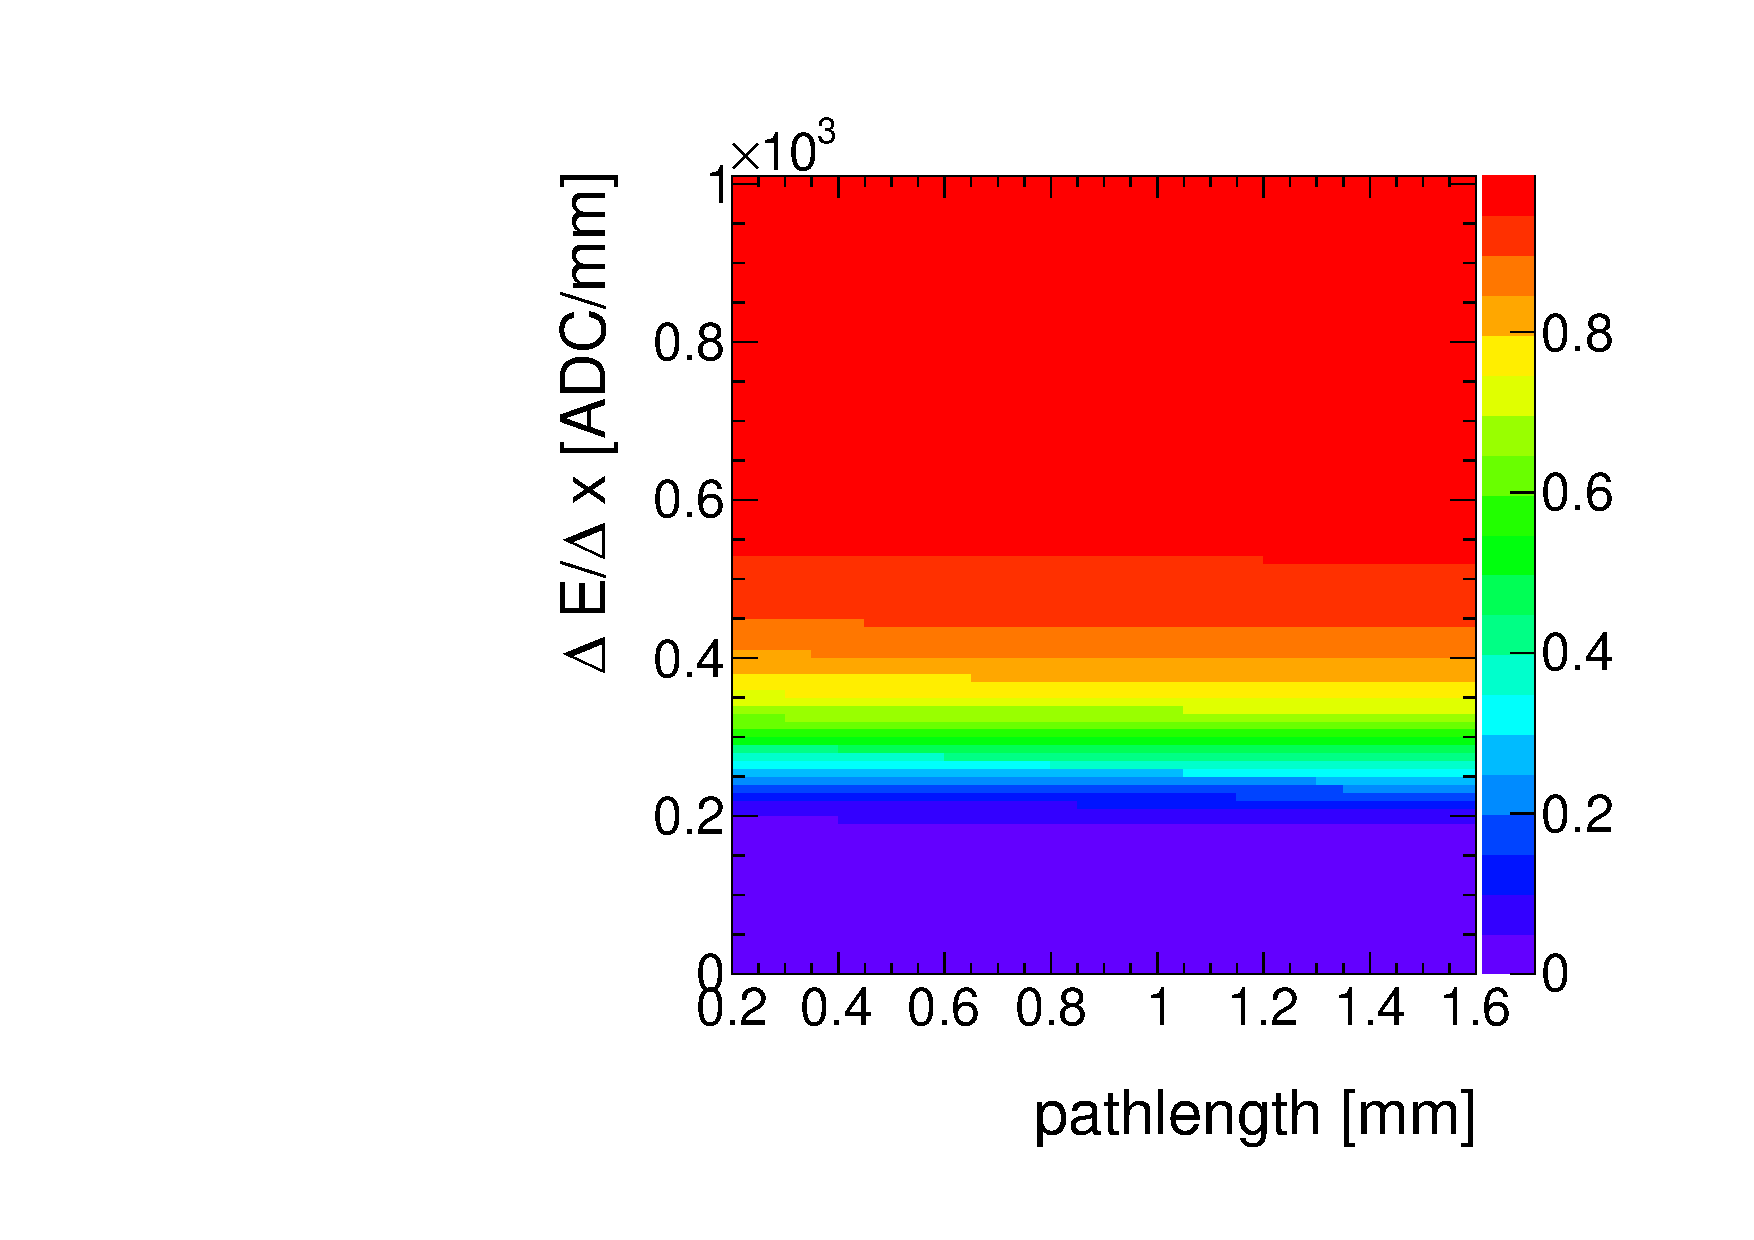
\includegraphics[width=0.49\textwidth]{figures/analysis_2/PixelCalibration/Discriminator_template_data_pixel_2012.pdf}
    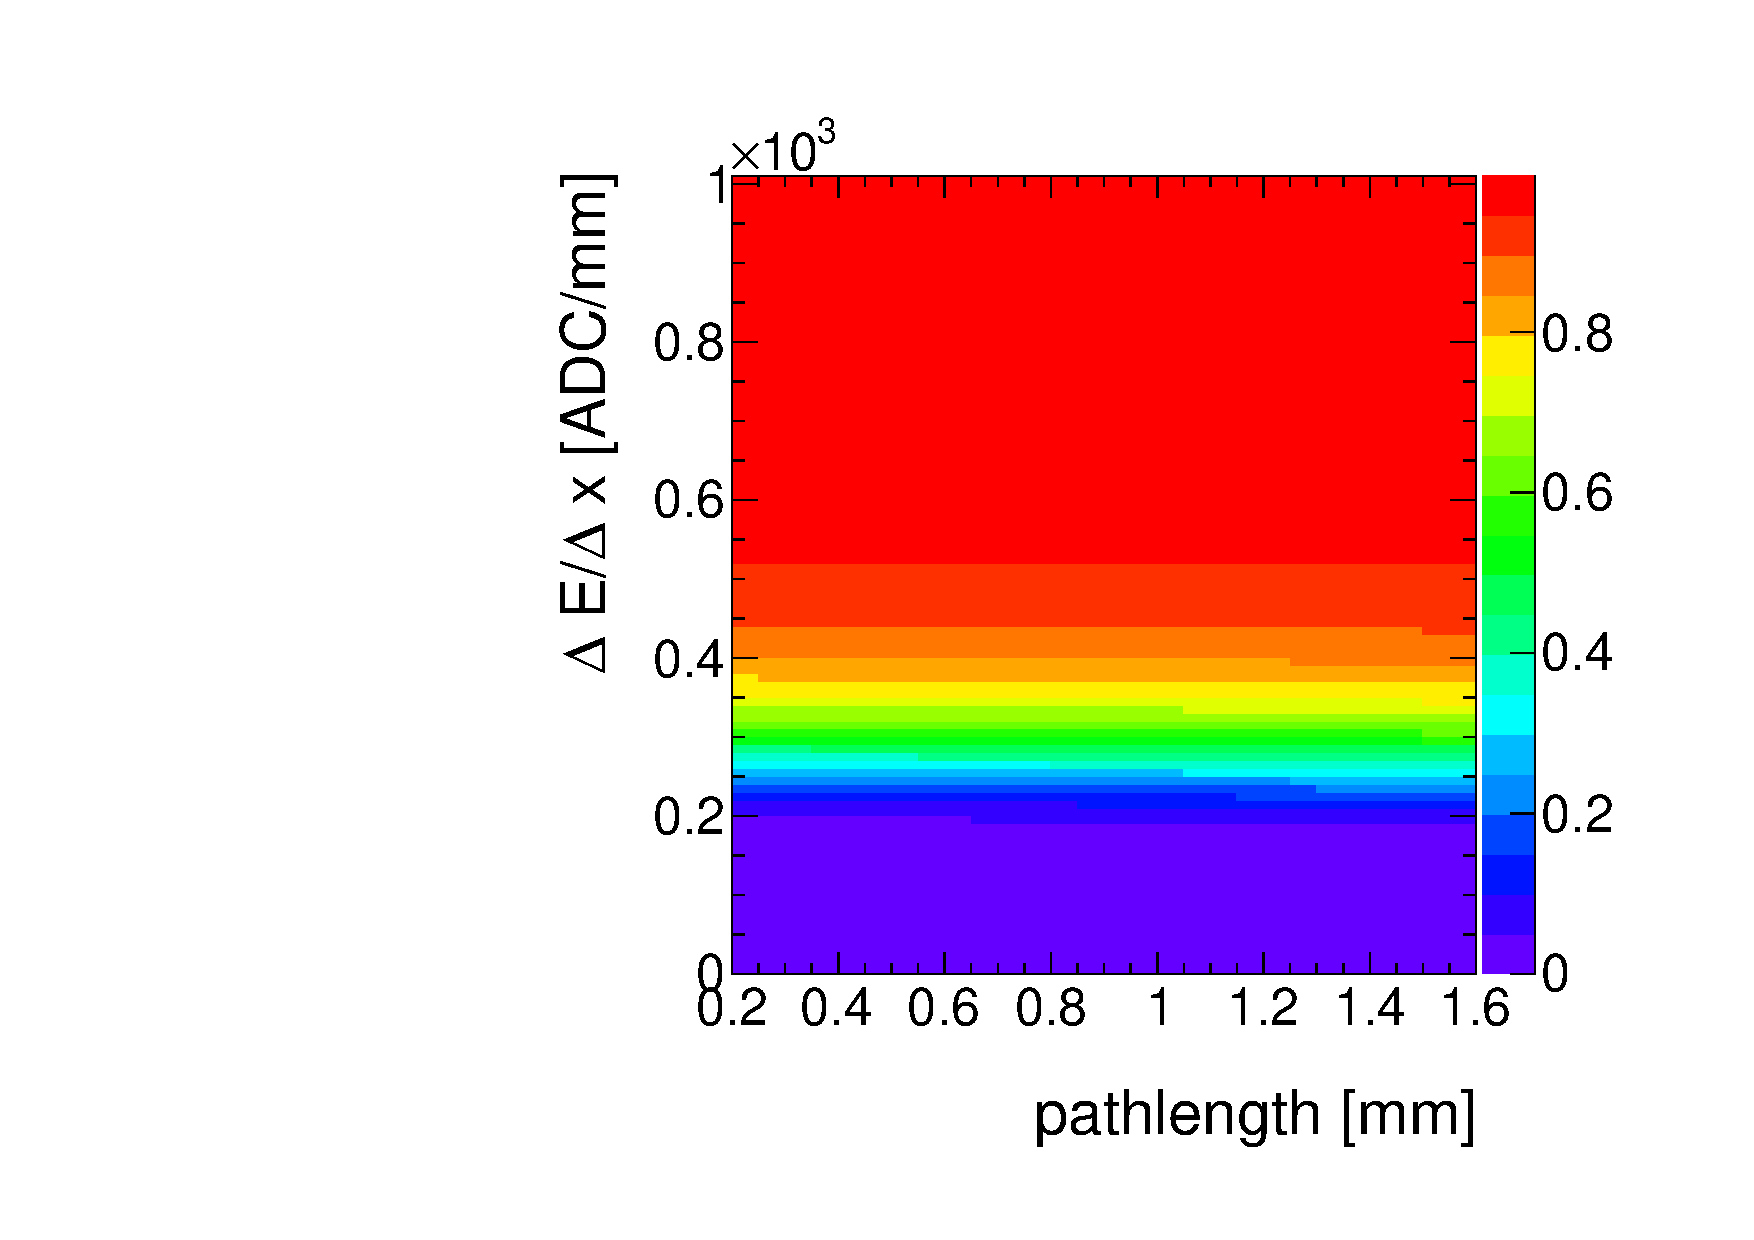
\includegraphics[width=0.49\textwidth]{figures/analysis_2/PixelCalibration/Discriminator_template_mc_pixel_2012.pdf}
  \end{tabular}
  \caption{Cumulative probability for a MIP to release a $\Delta E/ \Delta x$ (y-axis) vs. the path length (x-axis) in data (left) and simulation (right) for the pixel tracker based on the ``minimum bias'' sample.}
 % \vspace{60pt}
  \label{fig:ProbabilityTemplate}
\end{figure}

\begin{figure}[!bt]
%\vspace{10pt}
  \centering 
  \begin{tabular}{c}
    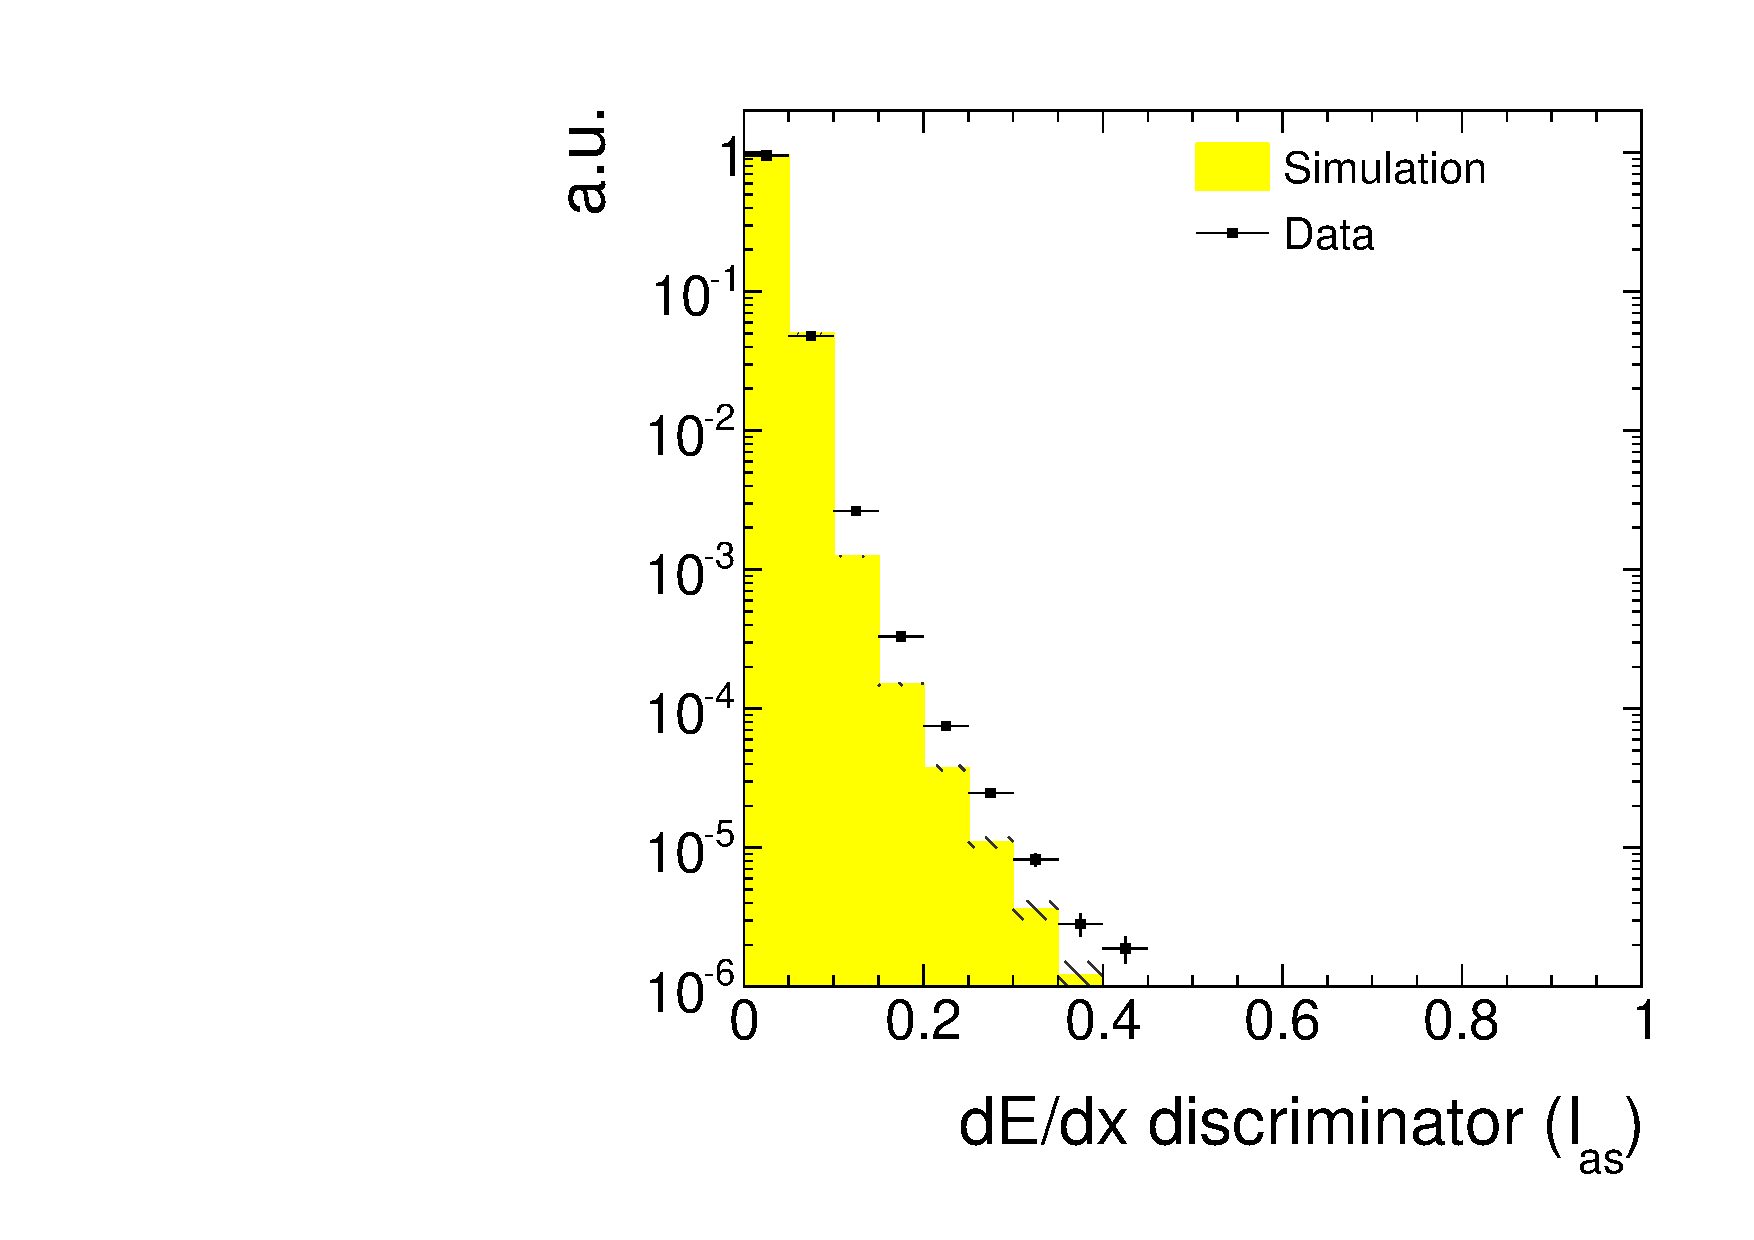
\includegraphics[width=0.49\textwidth]{figures/analysis_2/PixelCalibration/htrackASmiSmallRange_log_MIPs.pdf}
  \end{tabular}
  \caption{Normalised \ias distribution for MIPs from the minimum bias sample in data and simulation for high-quality (high purity as defined in \cite{bib:CMS:Tracking_2010}, a minimum number of eight hits and no missing inner and middle hits) tracks with $p>5\gev$ and $|\eta|<2.1$.}
  \label{fig:Data-MC-Dedx_MIPs}
\end{figure}
\dedx shows good agreement in data and simulation for $\ias<0.1$.
For larger values, \ias shows a larger decrease in simulation than in measured data.
For this reason a data-based approach for analyses exploiting \dedx information is needed.\\

\section{Discrimination improvements}
\label{sec:DiscriminationImprovements}
The goal of including the pixel energy information is to increase the discrimination power of \ias between background and signal tracks, especially for shorter lifetimes.
In Fig.~\ref{fig:MIPs-Signal-Dedx} (left), a comparison of the shapes of the energy release by MIPs and by signal tracks in simulation is shown (details about the simulated samples can be found in the next section Section~\ref{sec:SignalSamples}).
\begin{figure}[!t]
  \centering 
  \begin{tabular}{c}
    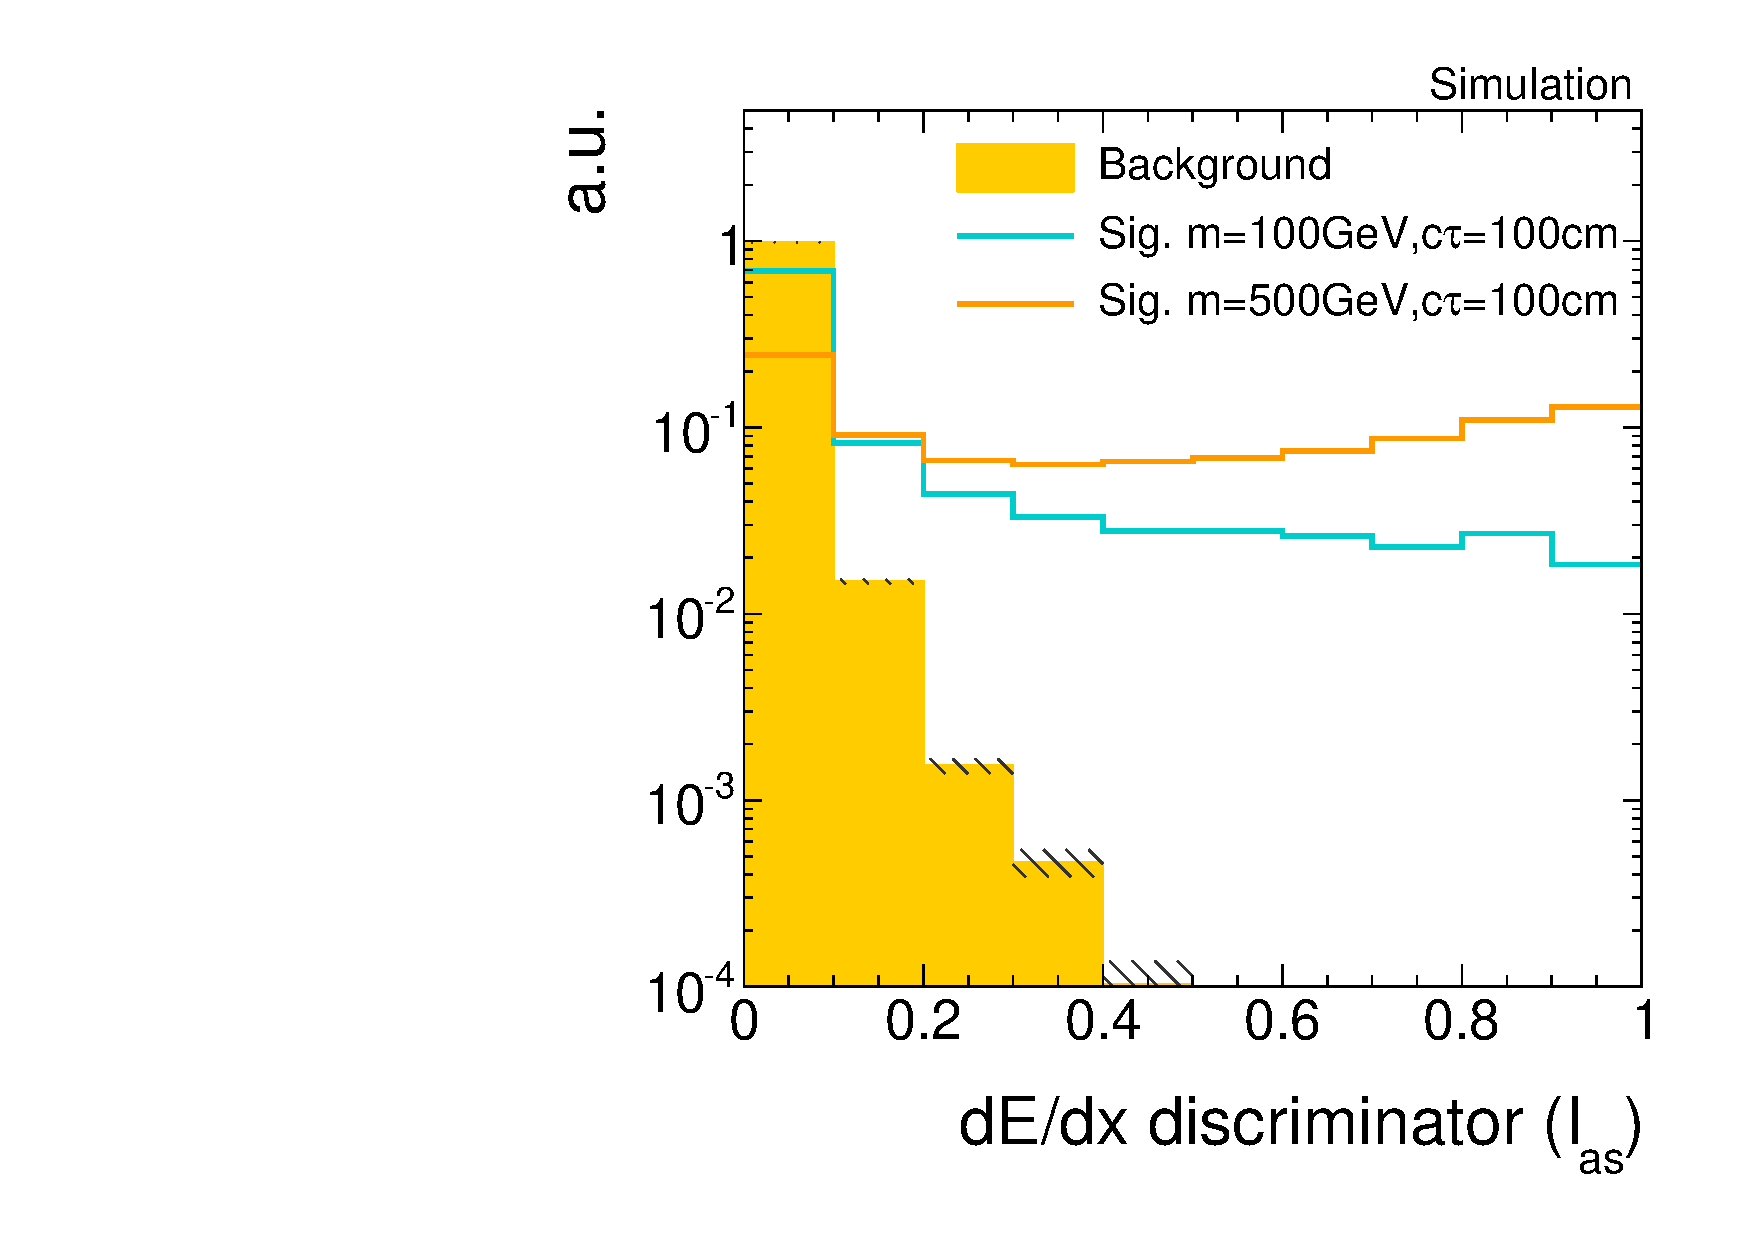
\includegraphics[width=0.49\textwidth]{figures/analysis_2/PixelCalibration/htrackASmiSmallRange_log_chiTracksGoodQualitySelection_2Signal_ttjets.pdf}   
    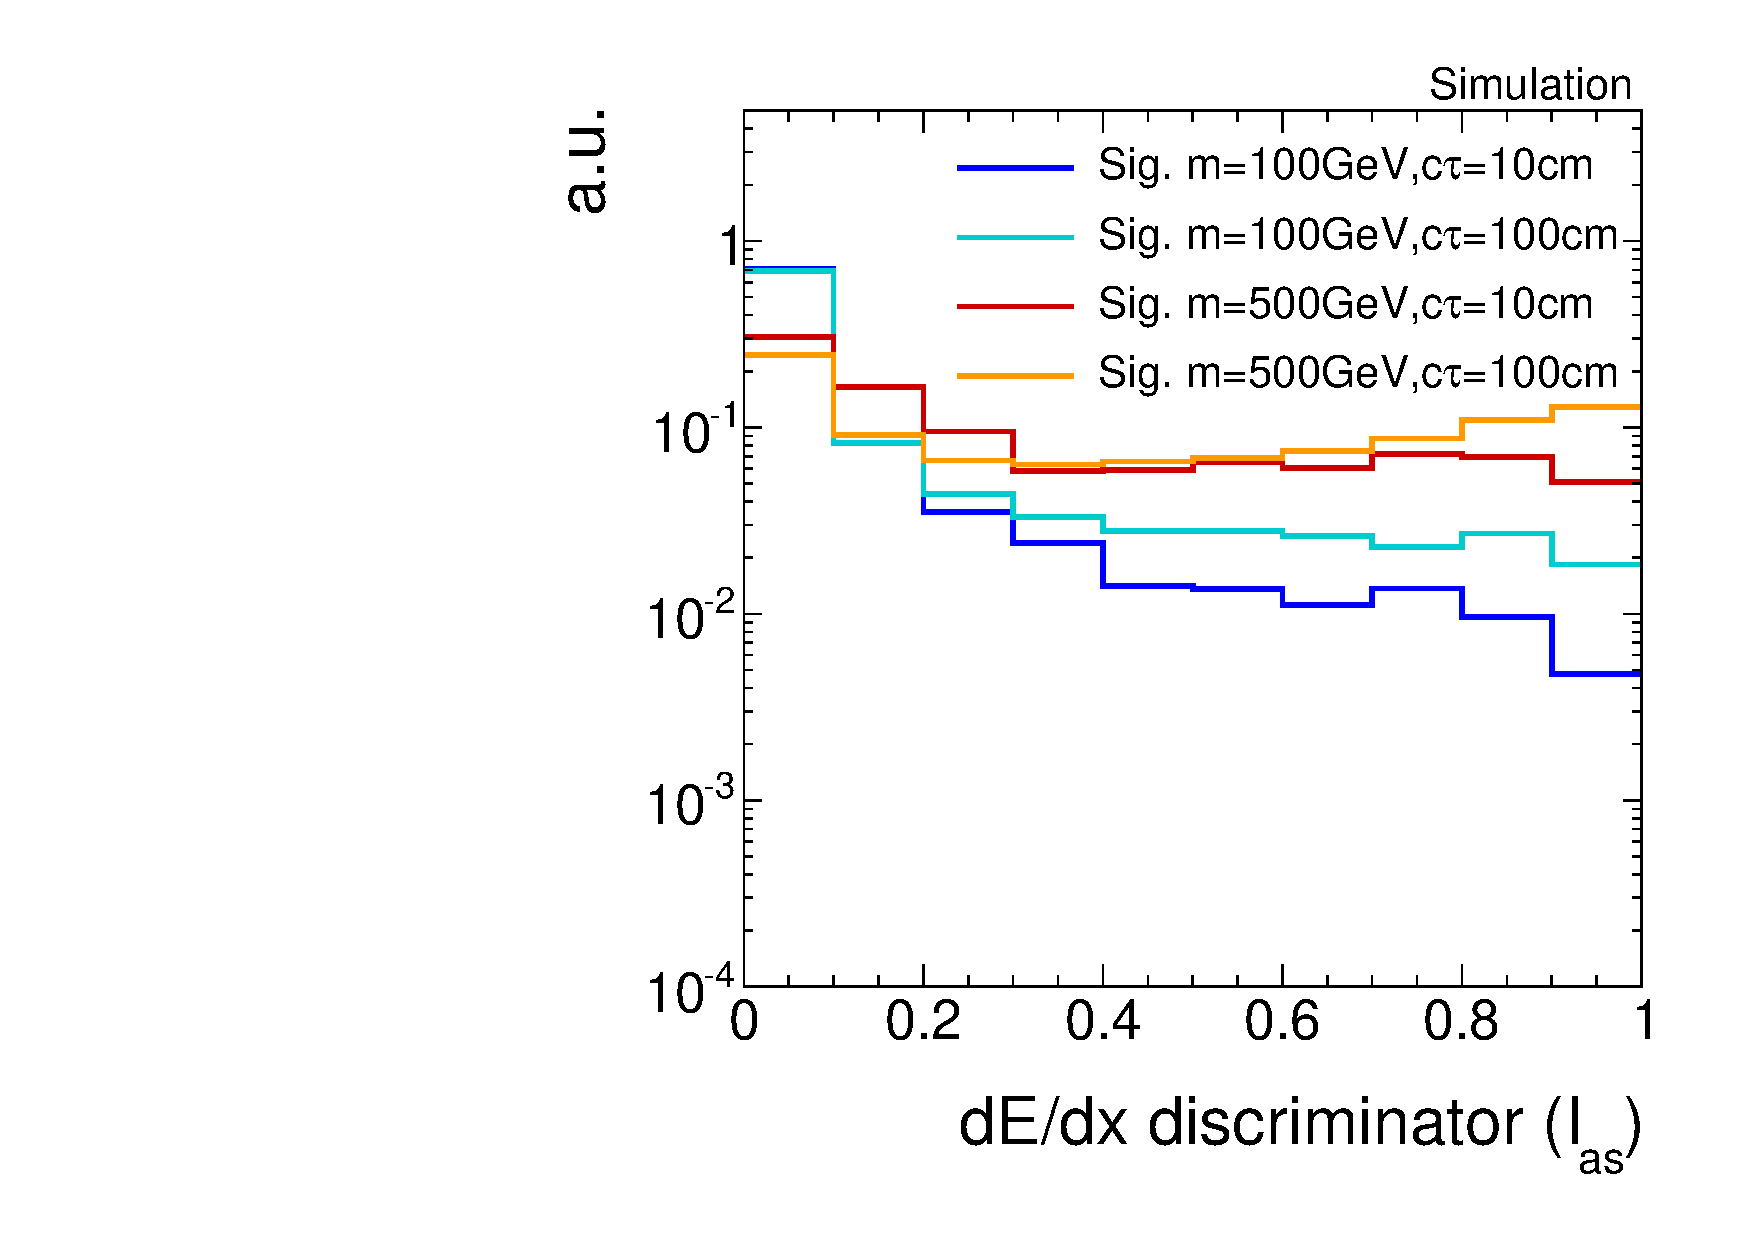
\includegraphics[width=0.49\textwidth]{figures/analysis_2/PixelCalibration/htrackASmiSmallRange_log_chiTracksGoodQualitySelection_4Signal.pdf}
  \end{tabular}
  \caption{Normalised \ias distribution for simulated background and signal tracks (left) and for four different signal models (right) 
           for high-purity tracks (as defined in \cite{bib:CMS:Tracking_2010}) with \pt$>10\gev$ and $|\eta|<2.1$.
           For the illustration of the background tracks' spectrum simulated $t\bar{t}$+jets events are used (more information about this sample is given in Chapter~\ref{ch:SimulatedSamples}).}
  \label{fig:MIPs-Signal-Dedx}
\end{figure} 
It can be seen, that the \ias distributions of the signal models show a larger tail towards $\ias=1$, whereas the \ias of the background is rapidly falling.

In the right part of Fig.~\ref{fig:MIPs-Signal-Dedx}, a comparison of the \ias distributions of four different signal models is shown.
Charginos with longer lifetimes have a more pronounced tail toward $\ias=1$.
This can be understood with the help of Eq.~\eqref{eq:Landau_Vavilov_Bichsel}, where the influence of the velocity ($\beta$) on the ionisation loss can be seen.
The velocity distribution of the charginos is mostly affected by the mass of the chargino.
However, also for charginos with same mass, the velocity is higher in average for shorter lifetimes.
This is caused by the fact, that for shorter lifetimes (\eg $\ctau=10\cm$), already a sizable fraction of the charginos decay before reaching the tracker system.
The probability of reaching the detector increases for higher velocities because of the boost, which can be clearly seen at the survival probability
\begin{equation}
P \left( t \right) = e^{-\frac{t}{\gamma \tau}}.
\end{equation} 
This means that the track reconstruction/selection lead to a biased average $\beta$ for shorter lifetimes which in turn lead to lower values of \ias.

The \ias distribution is not only influenced by the velocity of a particle but also by the number of hits of a track.
The number of measurements in the tracker system defines the influence of single fluctuations in $\Delta E/\Delta x$ on the \ias discriminator, because of the long right tail of the Landau distribution.
A low number of hits, therefore, leads to higher \ias values.
This effect is also visible in Fig.~\ref{fig:MIPs-Signal-Dedx} (right). 
The small surplus for lower lifetimes between 0.1 and 0.2 is caused by the smaller number of measurements for earlier decaying charginos.

%Thus, \ias for charginos with lower lifetimes are affected by two things: 
%First, due to the smaller number of measurements the chargino tends to higher \ias values.
%Second, low lifetimes charginos have in average a higher velocity leading to lower \ias values.
%Both effects can be seen in Fig.~\ref{fig:MIPs-Signal-Dedx} (right).
%The large tail for longer lifetimes is caused by the lower velocities, but the small surplus for lower lifetimes between 0.1 and 0.2 is caused by the smaller number of measurements for earlier decaying charginos.\\


Finally, the impact of the additional $\Delta E/\Delta x$ information from the pixel tracker on the selection efficiency of signal and background tracks is quantified.
Figure~\ref{fig:ROCplots} shows the signal selection efficiency against the background selection efficiency for different selection cuts in \ias, once including the pixel information and once without it.
\begin{figure}[!t]
  \centering 
  \vspace{50pt}
  \begin{tabular}{c}
    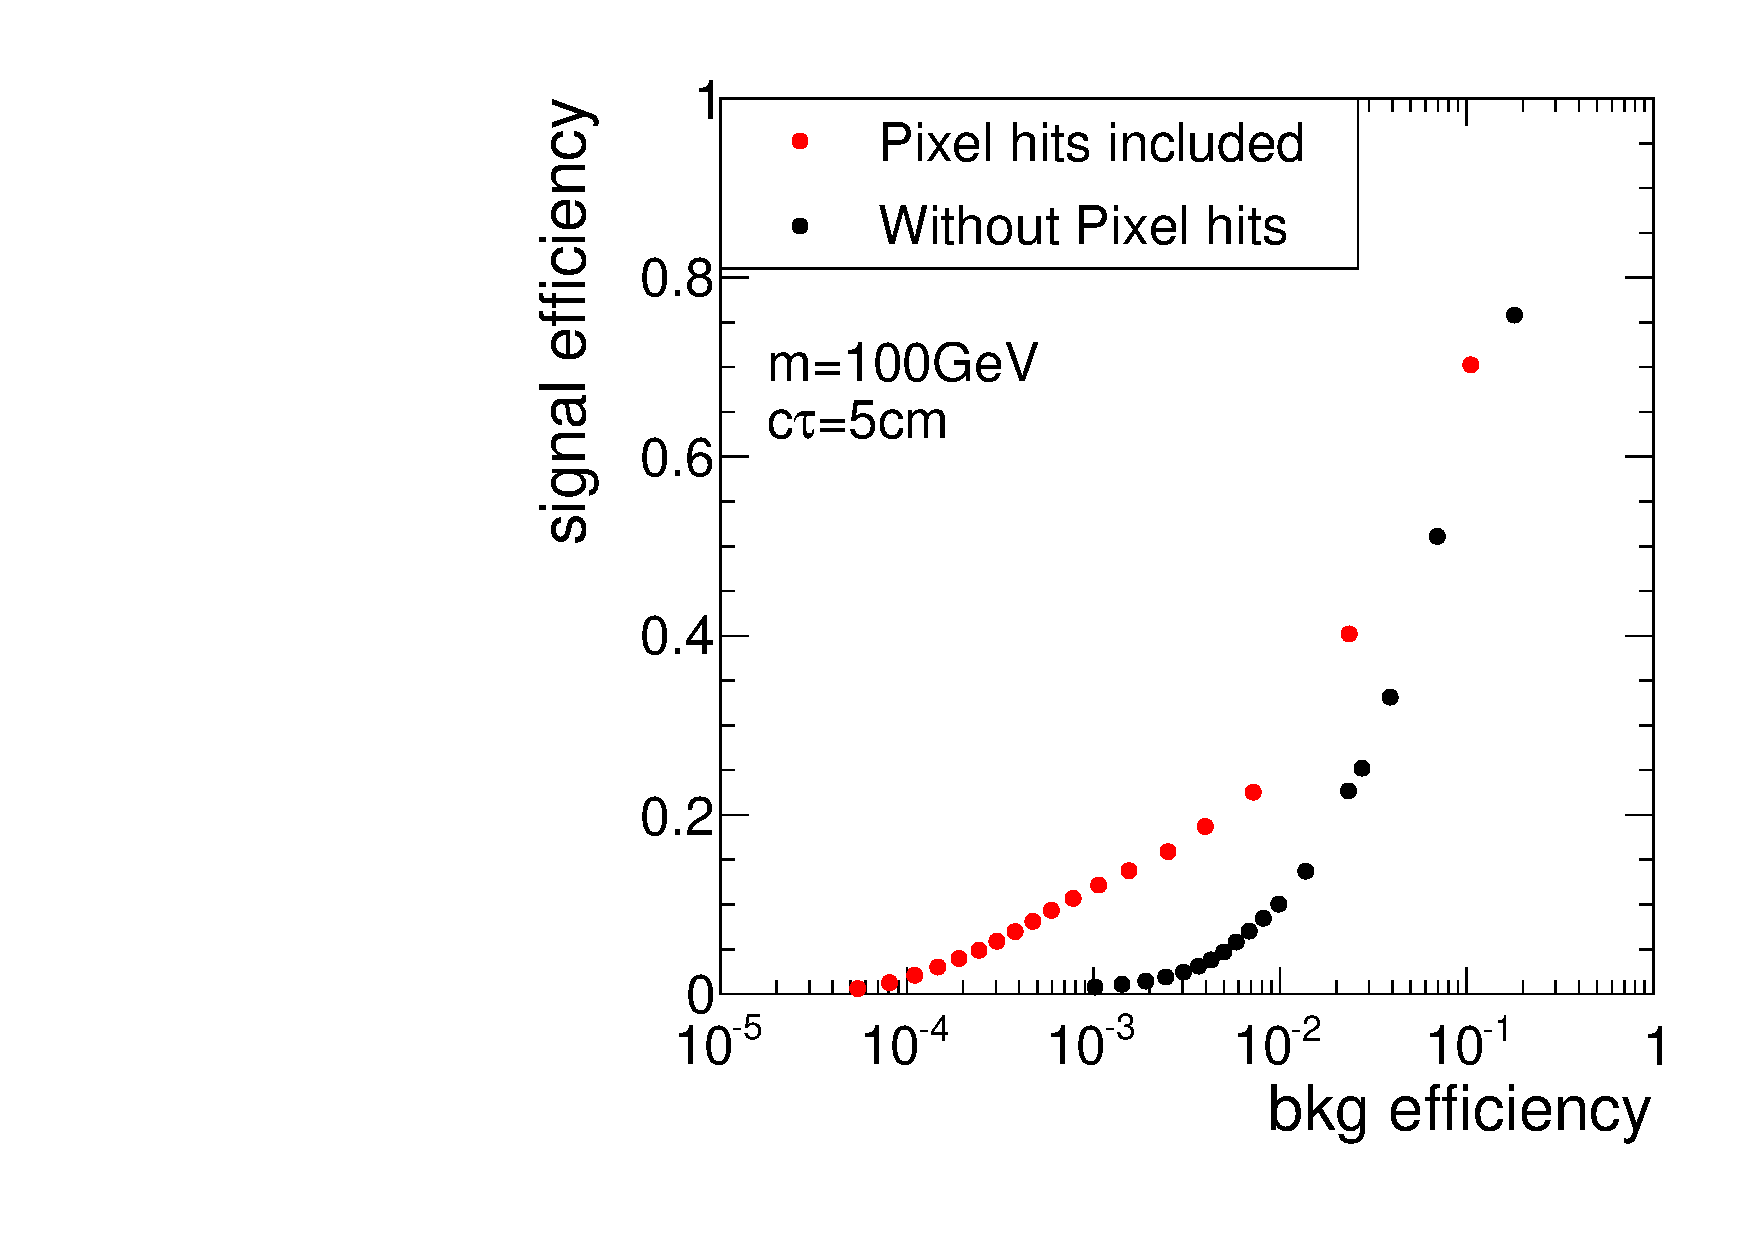
\includegraphics[width=0.49\textwidth]{figures/analysis/rocplot_wjets_mass_100GeV_ctau_5cm.pdf} 
    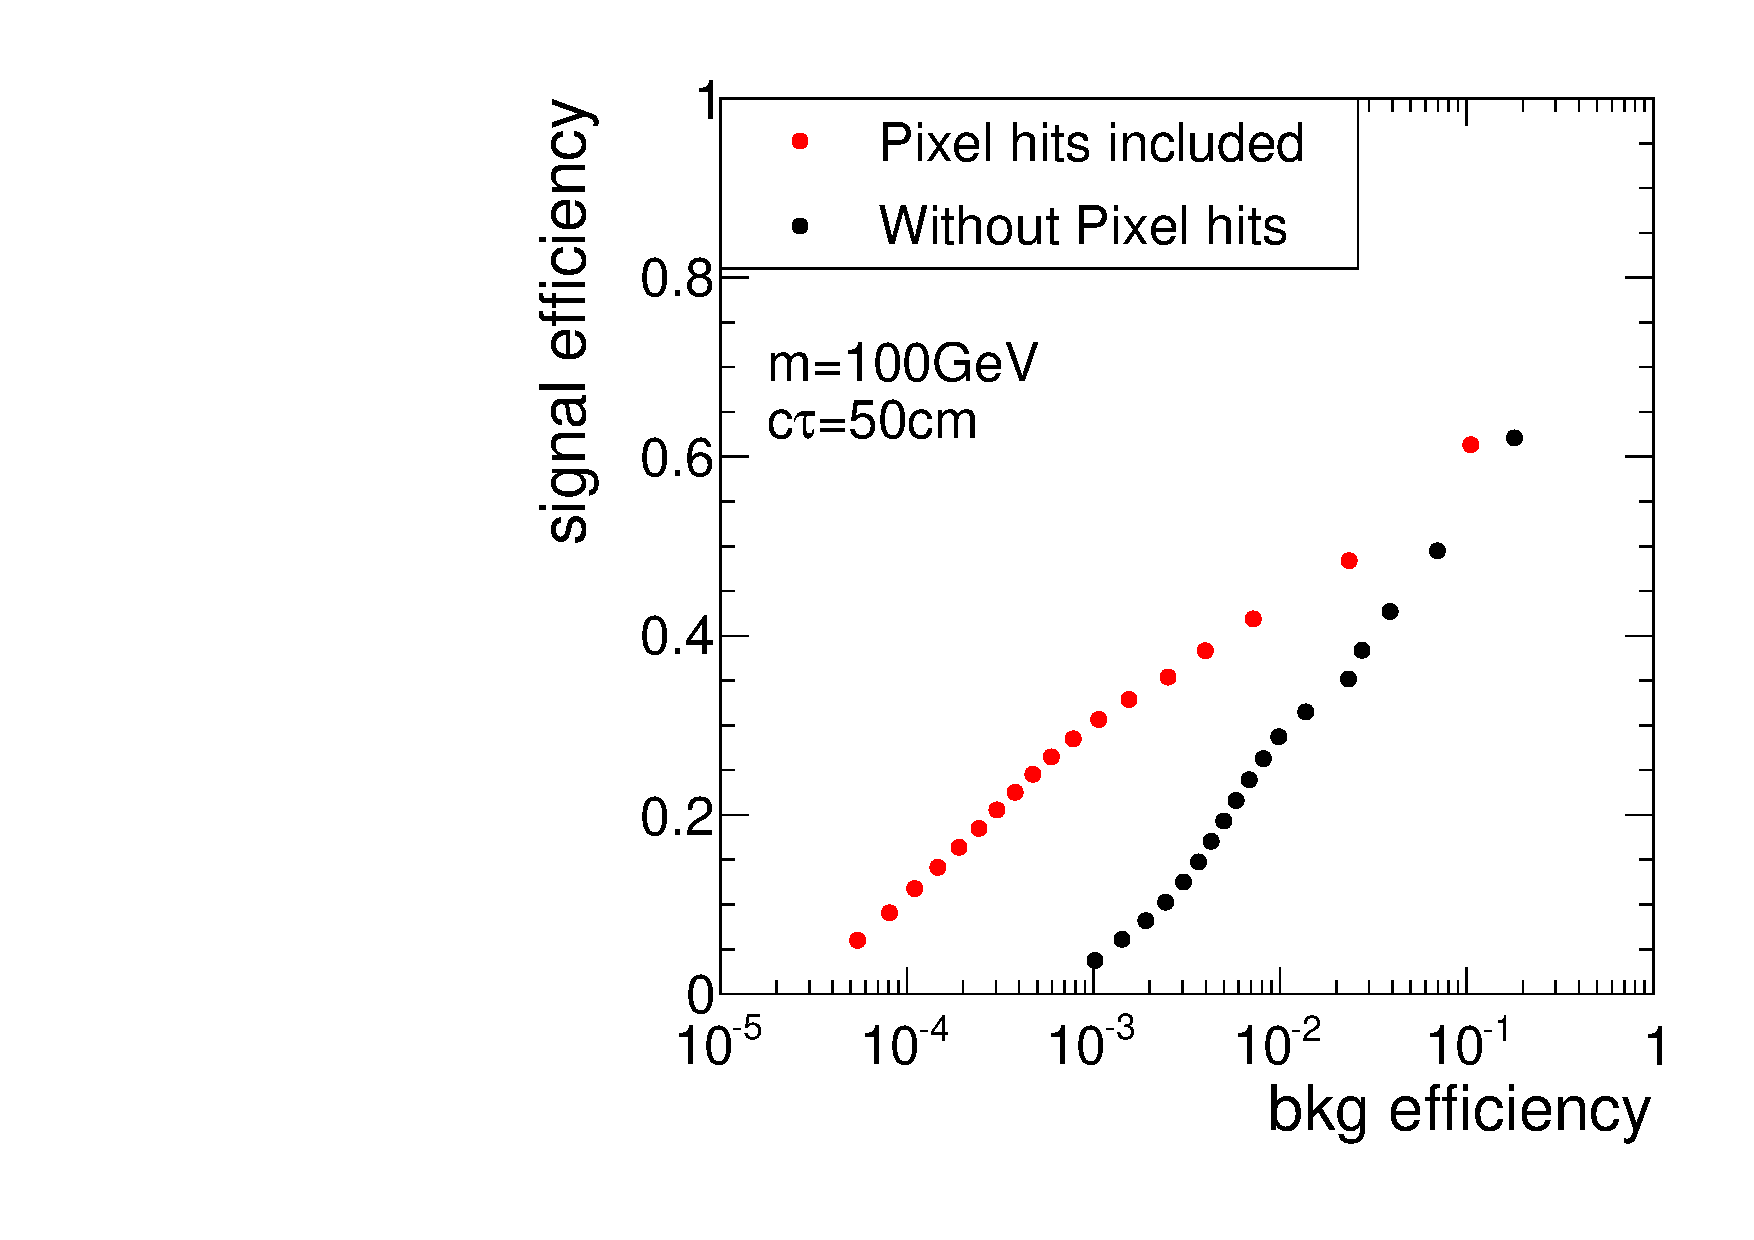
\includegraphics[width=0.49\textwidth]{figures/analysis/rocplot_wjets_mass_100GeV_ctau_50cm.pdf} \\
    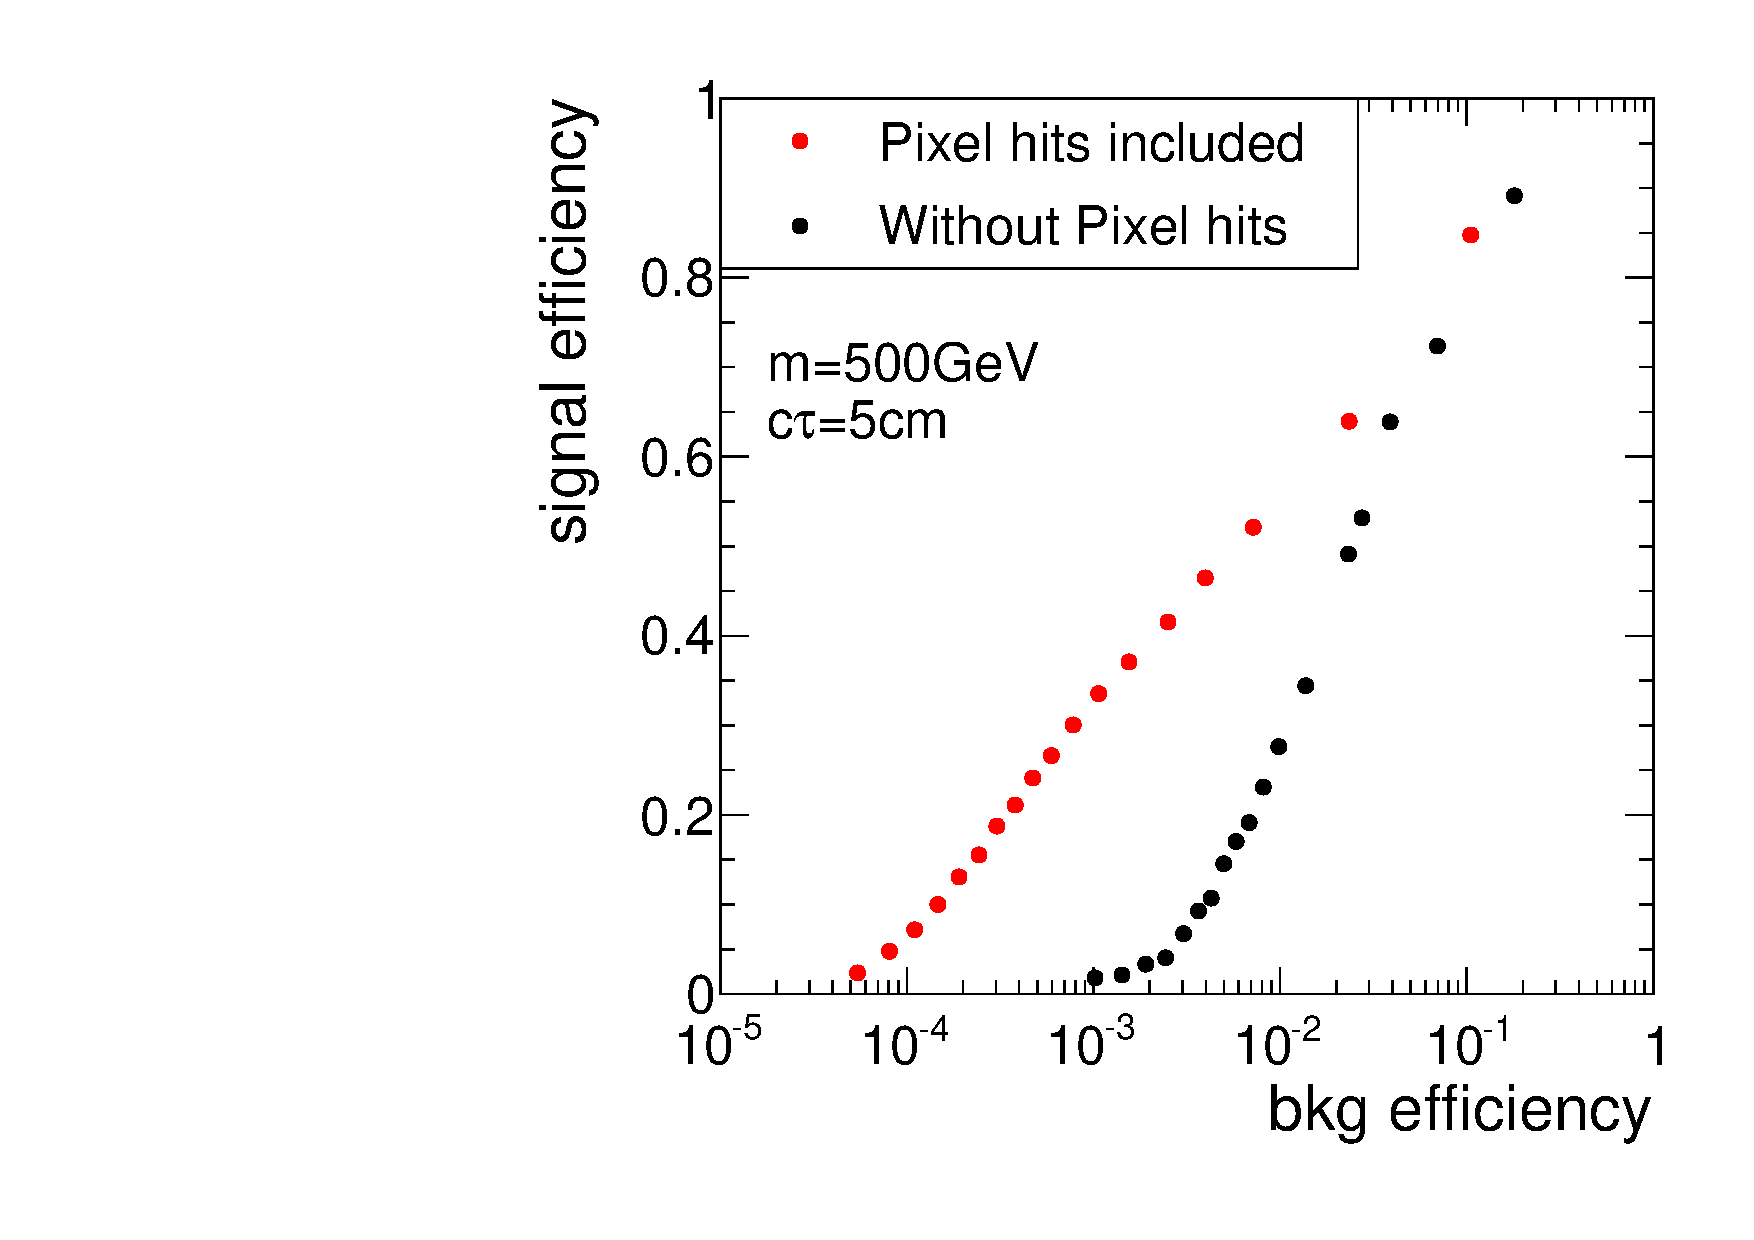
\includegraphics[width=0.49\textwidth]{figures/analysis/rocplot_wjets_mass_500GeV_ctau_5cm.pdf} 
    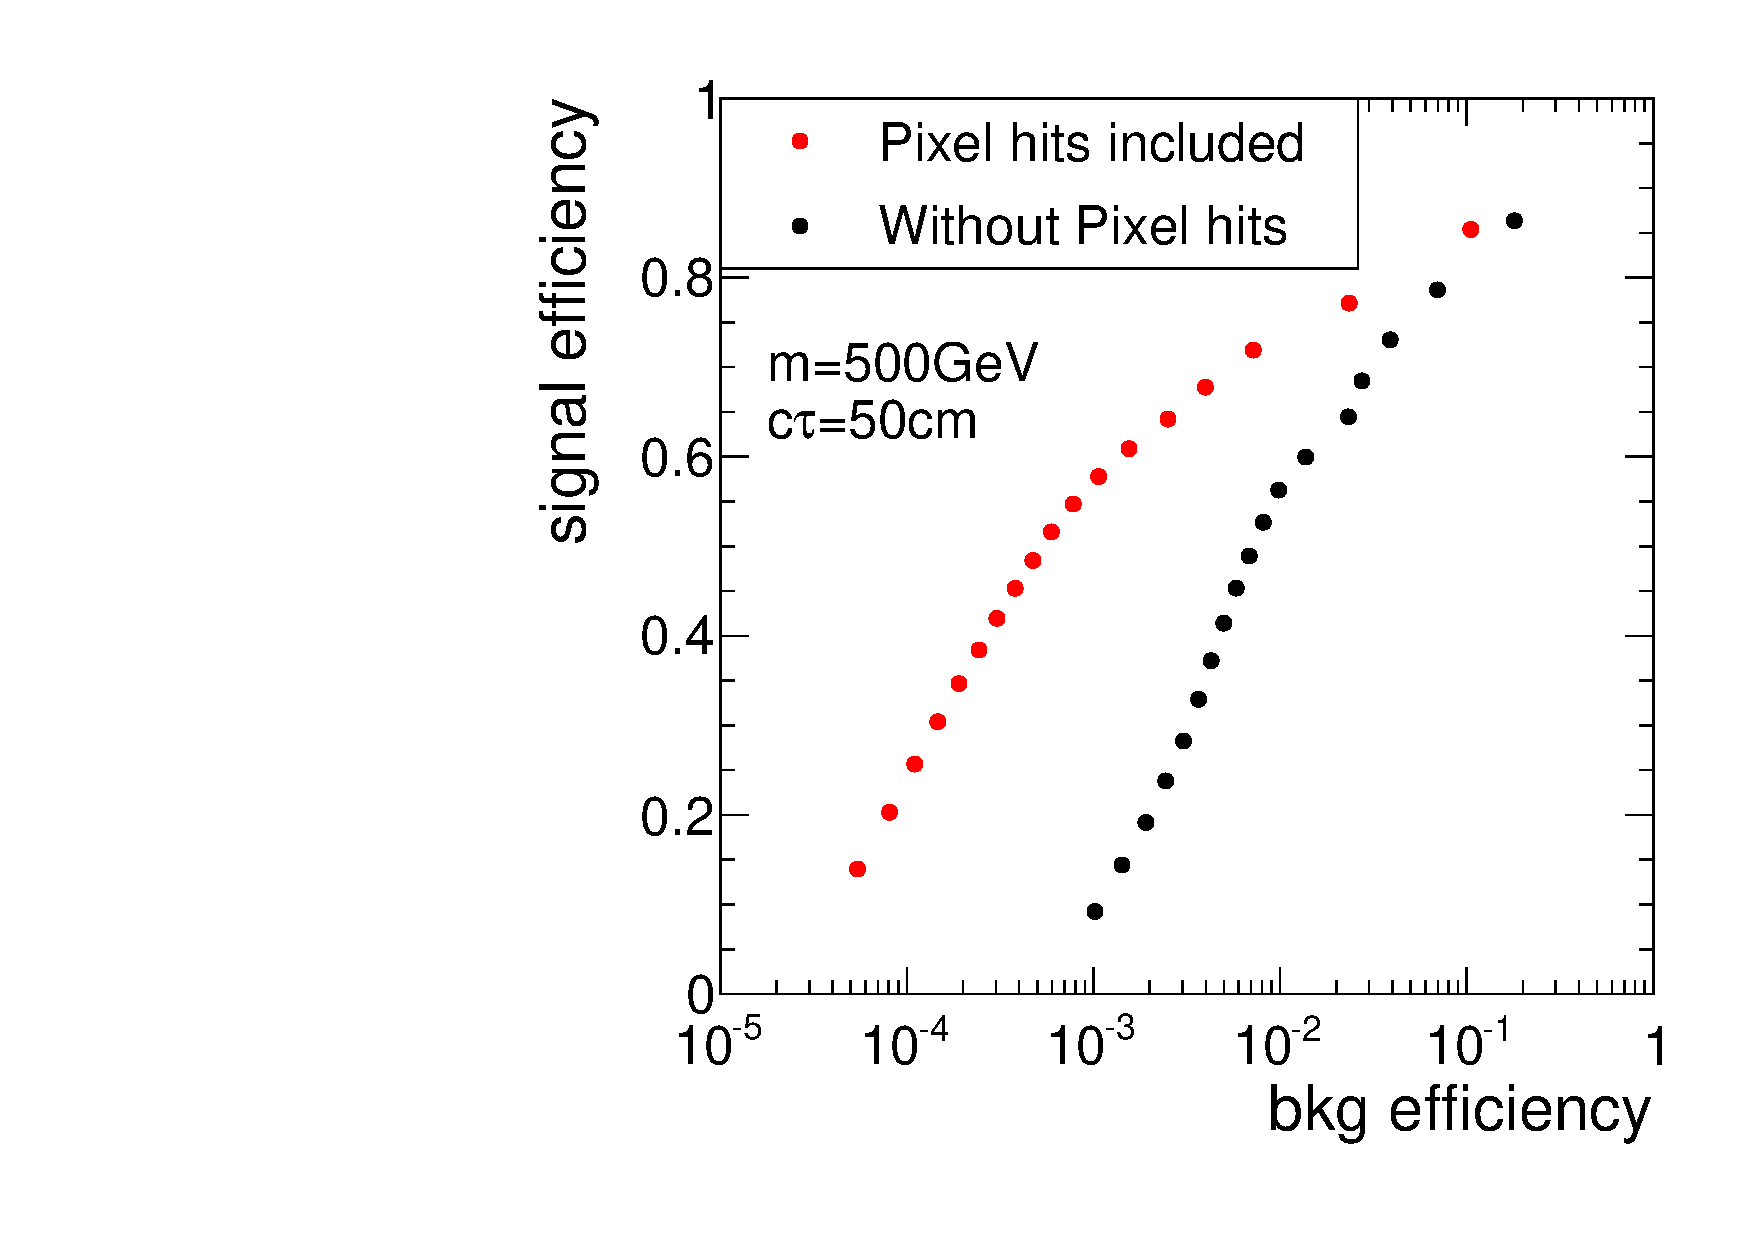
\includegraphics[width=0.49\textwidth]{figures/analysis/rocplot_wjets_mass_500GeV_ctau_50cm.pdf}
  \end{tabular}
  \caption{Signal selection efficiency vs. background selection efficiency with (red) and without (black) pixel information.
           Each point correspond to one selection cut in \ias.
           The figure is based on a simulated \WJets sample and a simulated signal sample with chargino-chargino production, both subject to a selection of high-quality tracks (without a selection on \nhits) with $\pt>10\gev$.}
  \vspace{40pt}
  \label{fig:ROCplots}
\end{figure} 
The background selection efficiency is estimated with simulated $W$+jets  events but was additionally checked on simulated $t\bar{t}$+jets  and QCD-multijet events 
(further information about the simulated samples can be found in the next Chapter~\ref{ch:SimulatedSamples}).
No significant difference between these processes in the background selection efficiency was observed.

The signal selection efficiency and the background suppression depend on the mass and the lifetime of the charginos.
The improvement of the discriminating power is much more pronounced for higher chargino masses.

It can be seen that the inclusion of the pixel information increases the background suppression for a given signal efficiency throughout the investigated signal models.
This background suppression improvement is most pronounced for very tight cuts on \ias up to a factor of 20 and even more and still considerable for looser selections with signal efficiencies of around 40\% (factor of 10).
%%%%%%%%%%%%%%%%%%%%%%%%%%%%%%%%%%%%%%%%%%%%%%%%%%%%%%%%%%%%%%%%%%%%%%%%%%%%%%%%%%%%%%%%%%%%%%%%%%%%%%%%%%%%%%%%%%%%%%%%%%%%%%%%%%%%%%%%%%%%%%%%%%%%%%%%%%%%%%%%%%%%%%%%%%%%%%%%%%%%
%%%%%%%%%%%%%%%%%%%%%%%%%%%%%%%%%%%%%%%%%%%%%%%%%%%%%%%%%%%%%%%%%%%%%%%%%%%%%%%%%%%%%%%%%%%%%%%%%%%%%%%%%%%%%%%%%%%%%%%%%%%%%%%%%%%%%%%%%%%%%%%%%%%%%%%%%%%%%%%%%%%%%%%%%%%%%%%%%%%%
